\documentclass[a4paper,10pt]{article}

\usepackage{ucs}
\usepackage[utf8]{inputenc}
\usepackage[english]{babel}
\usepackage{fontenc}
\usepackage{graphicx}
\usepackage{longtable}
\usepackage{multirow}

\usepackage[dvips]{hyperref}

\date{13/06/2018}

\begin{document}
 \begin{center}
\begin{longtable}{|l|l|l|p{6cm}|}
\caption[RBP Motifs]{Sequence motifs for RNA Binding Proteins (RBPs) involved in alternative splicing. RBPs were selected for analysis in this study if
they had a well-defined position-specific binding matrix and a role in mediating alternative splicing was known from the literature. The consensus sequences
are shown using the IUPAC codes for positions in which multiple different nucleotides are observed; R (A or G);  Y (C or T); S (G or C); W (A or T);
K (G or T); M (A or C).} \label{tab:rbp-motif} \\

\hline \multicolumn{1}{|l|}{\textbf{RBP}} & \multicolumn{1}{c|}{\textbf{Consensus}}& \multicolumn{1}{c|}{\textbf{Logo}} & \multicolumn{1}{p{6cm}|}{\textbf{Function}} \\ \hline 
\endfirsthead

\multicolumn{4}{c}%
{{\bfseries \tablename\ \thetable{} -- continued from previous page}} \\
\hline \multicolumn{1}{|l|}{\textbf{RBP}} &
\multicolumn{1}{l|}{\textbf{Consensus}} &
\multicolumn{1}{l|}{\textbf{Motif}} &
\multicolumn{1}{p{6cm}|}{\textbf{Function}} \\ \hline 
\endhead

\hline \multicolumn{4}{|r|}{{Continued on next page}} \\ \hline
\endfoot

\hline \hline
\endlastfoot
SRSF1  &  GRAGGA &
 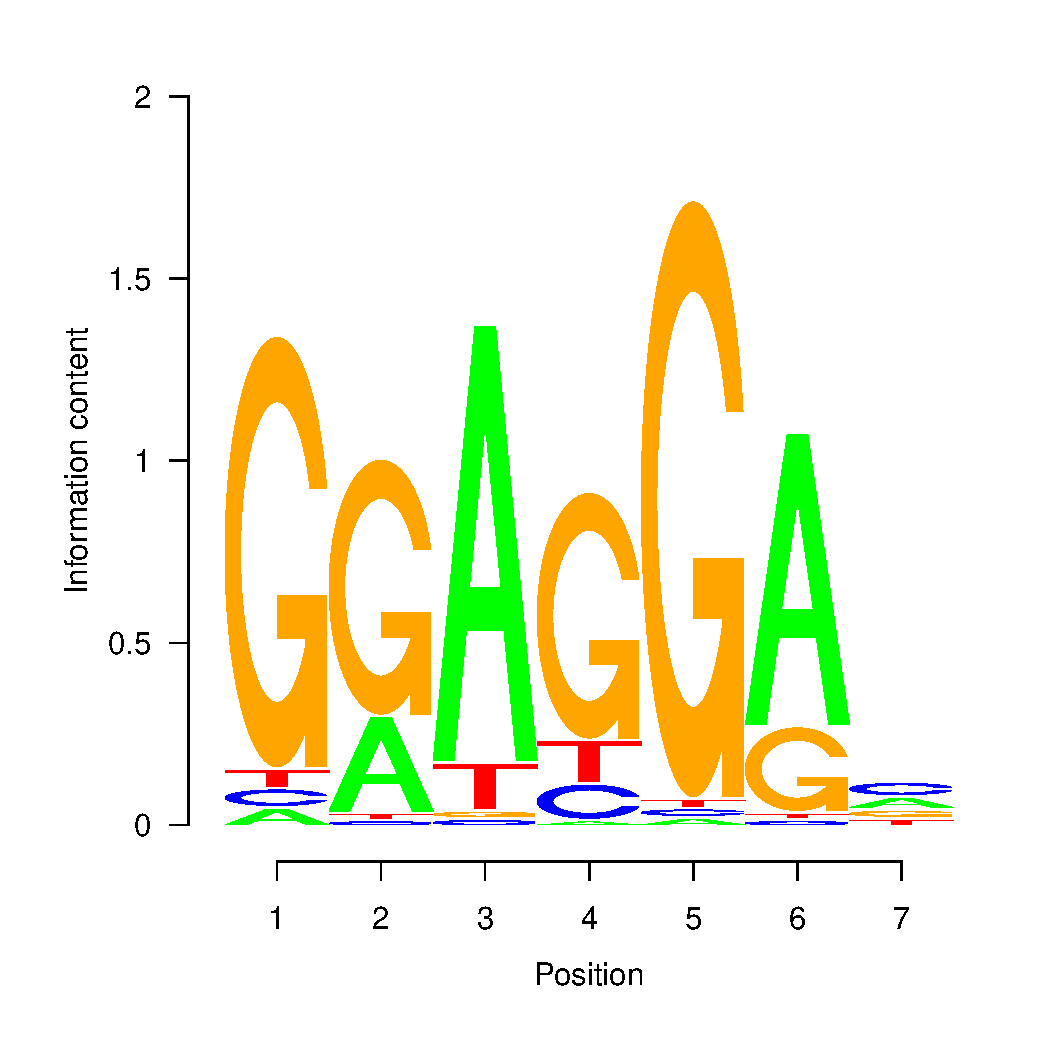
\includegraphics[height=0.8in]{./seqLogo/SRSF1_gragga.pdf}
 & \multirow{6}{6cm}{
 \textbf{SR Family} \newline 
 Serine and Arginine-rich (SR) proteins are key determinants of exon identity and function 
 as molecular adaptors, linking the pre-mRNA to the splicing machinery. SR proteins display
 a modular domain structure consisting of one to two amino- terminal RNA recognition motifs (RRMs) and a carboxyl-terminal domain rich in serine and arginine dipeptide repeats.
 SR proteins contribute to spliceosome assembly primarily through the recognition of exonic splicing enhancers (ESEs).
  SR proteins play a position- and context-dependent role in alternative splicing, and tend to act as enhancers of splicing when associated with exonic sequences, but function as silencers while binding to intronic sequences 
  downstream of the 5′ splice site~\cite{Howard2015}.
TODO -- find ref for  Usually promote inclusion of alternative exon by binding to enhancer elements
} \\
\cline{1-3}
SRSF2 & GGAGWD &
 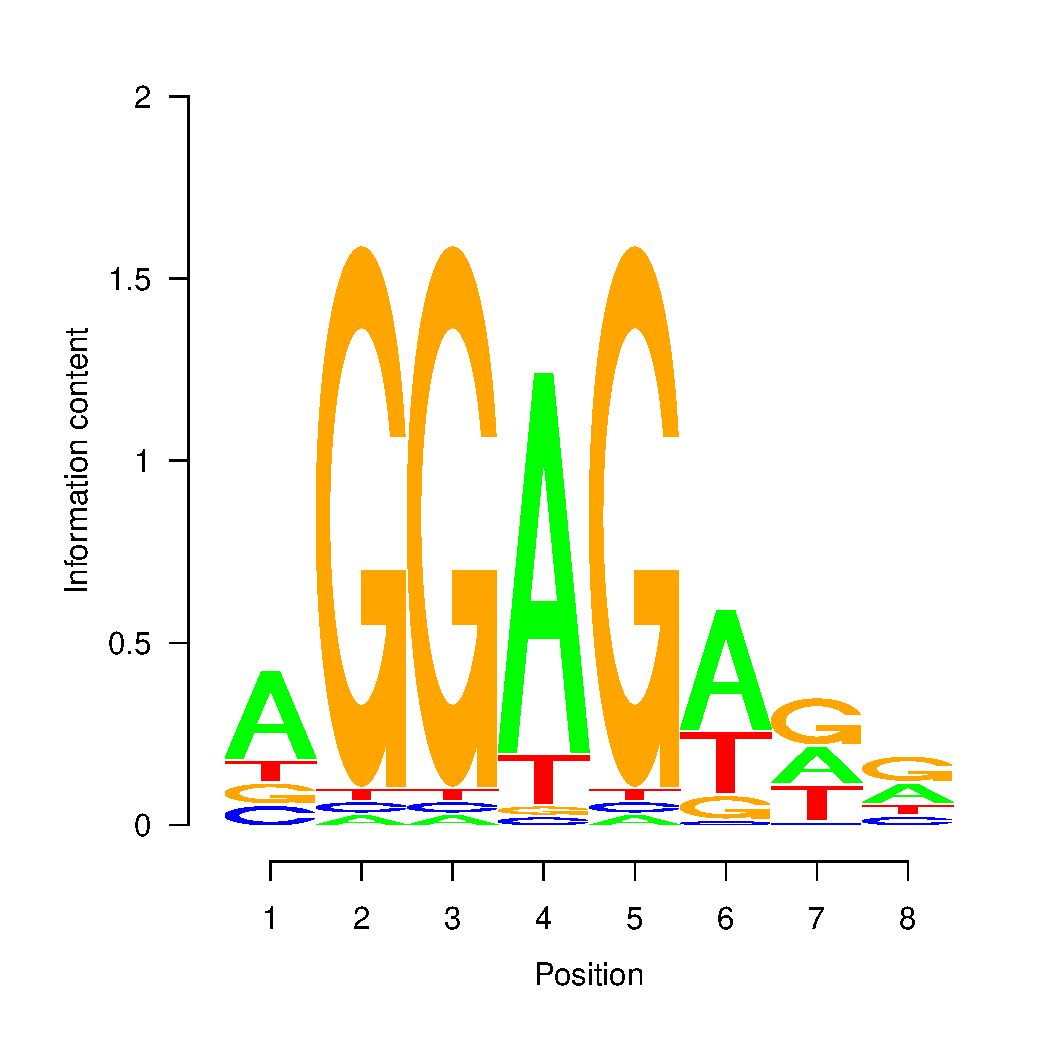
\includegraphics[height=0.8in]{./seqLogo/SRSF2_ggagwd.pdf}
 &  \\
 \cline{1-3}
SRSF7 & ACGACG &
 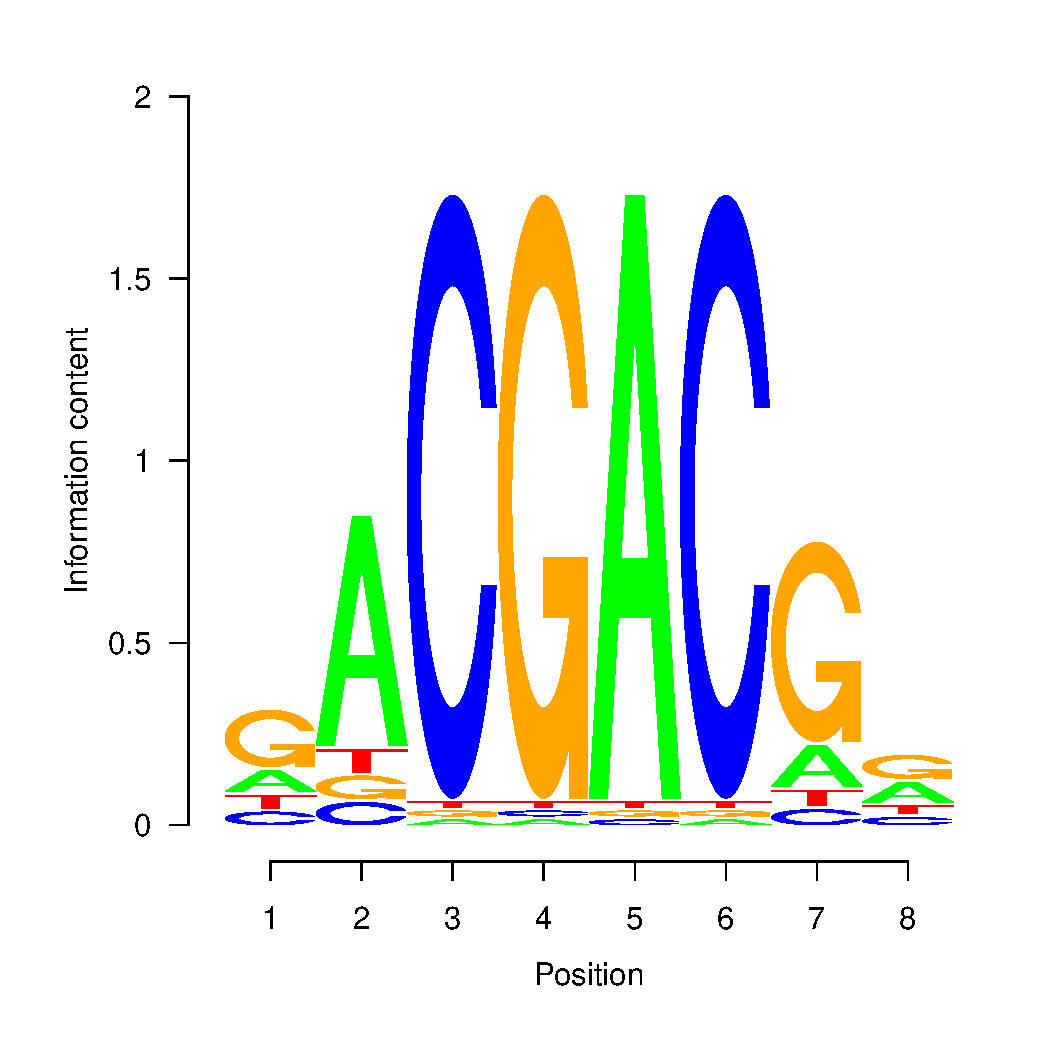
\includegraphics[height=0.8in]{./seqLogo/SRSF7_acgacg.pdf}
 &  \\
  \cline{1-3}
SRSF9 (a) & AKGAVMR &
 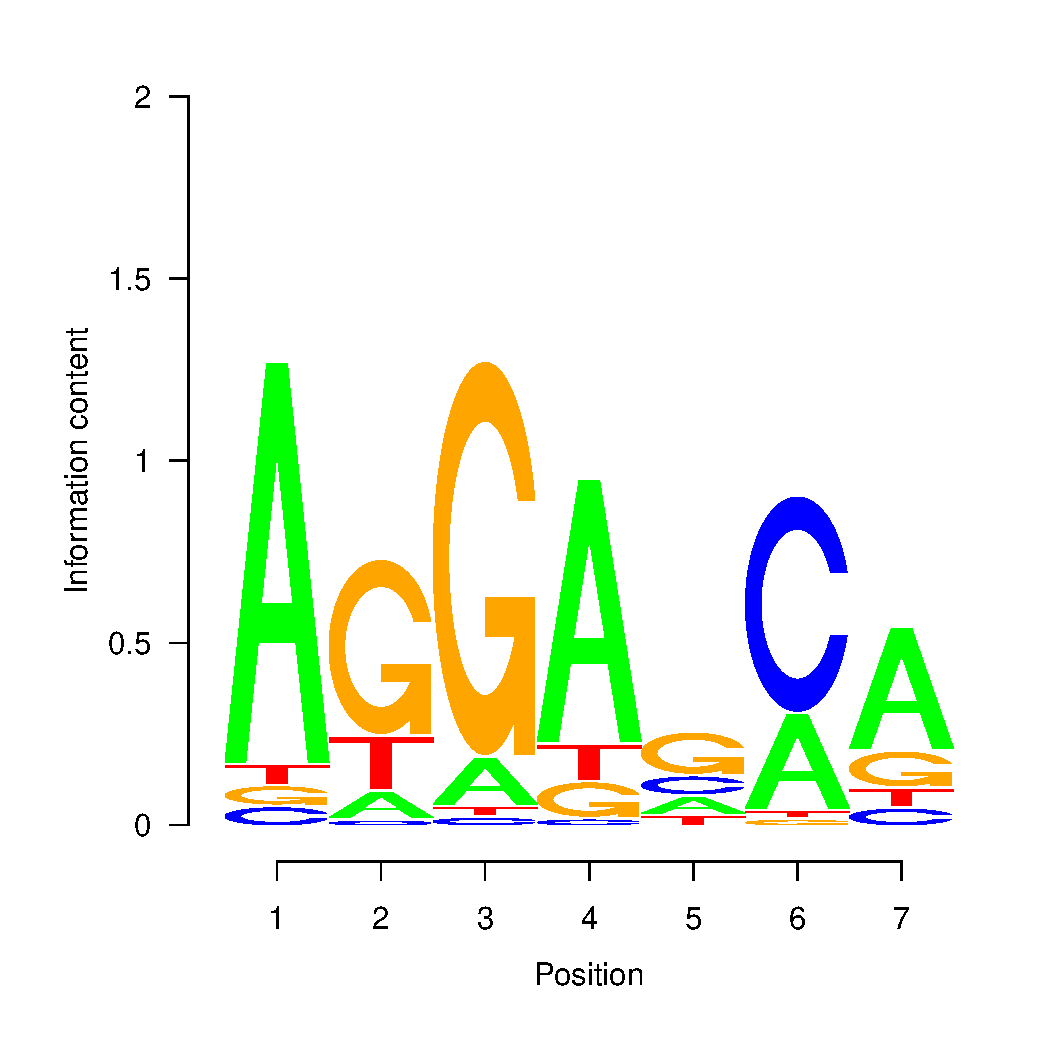
\includegraphics[height=0.8in]{./seqLogo/SRSF9_akgavmr.pdf}
 &  \\
   \cline{1-3}
SRSF9 (b)  &  KGRWGSM &
 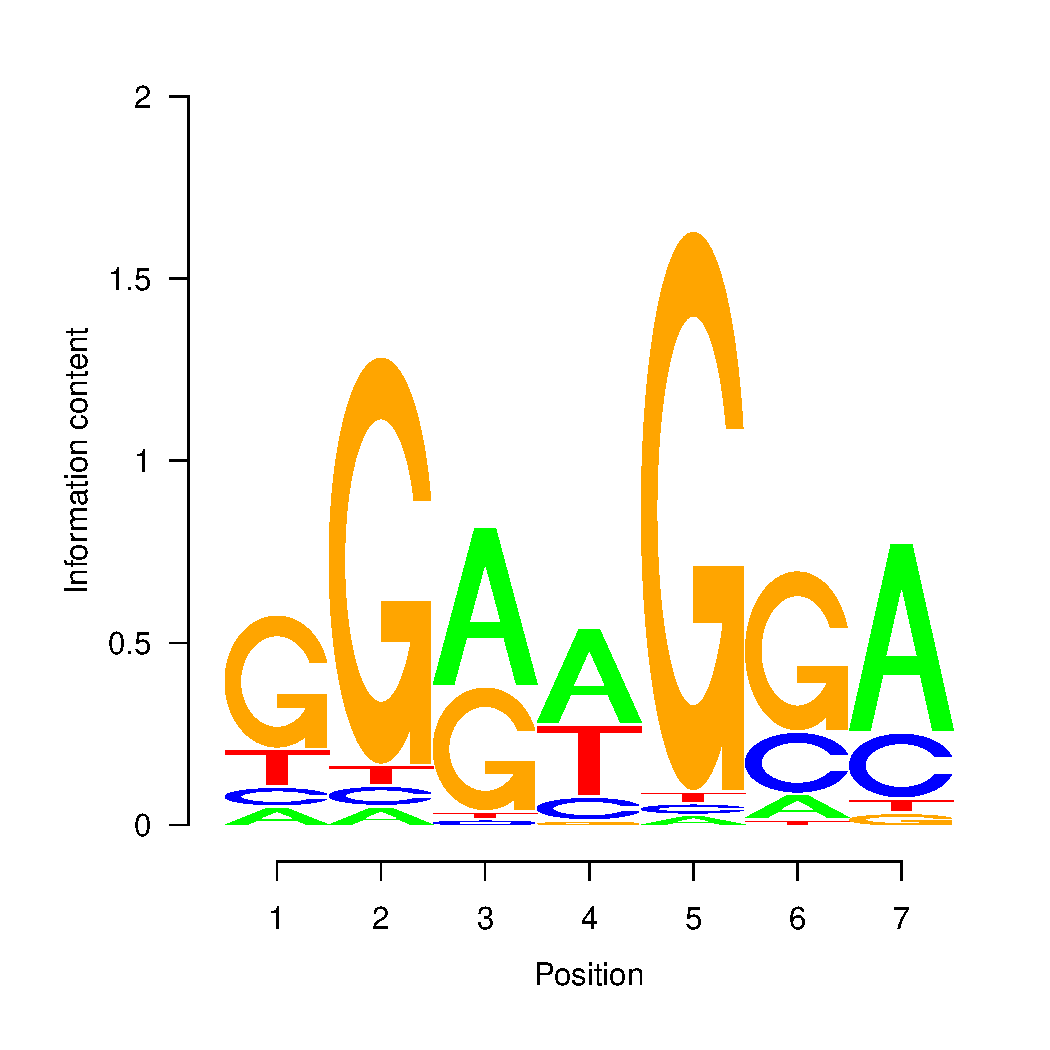
\includegraphics[height=0.8in]{./seqLogo/SRSF9_kgrwgsm.pdf}
 &  \\
 \cline{1-3}
SRSF10 & AGAGAVM & 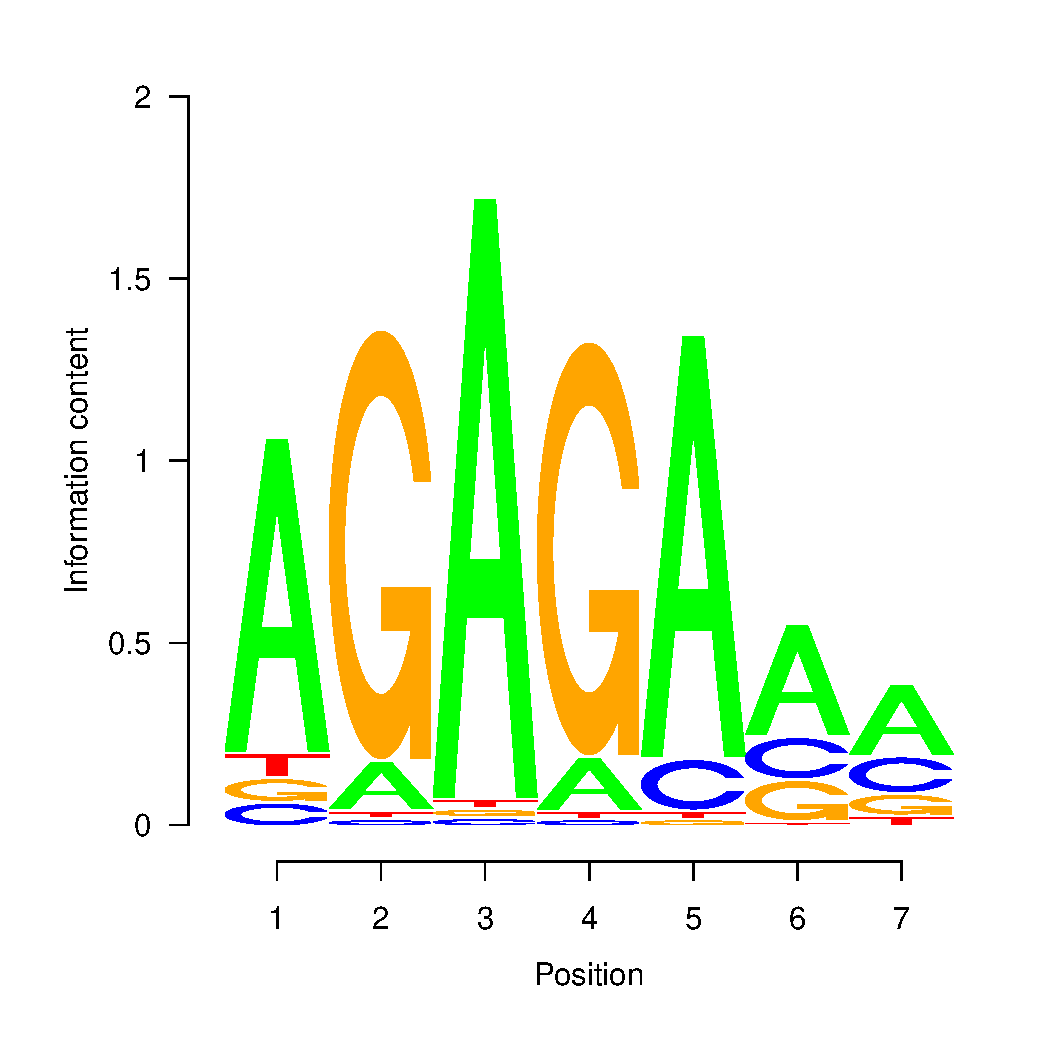
\includegraphics[height=0.8in]{./seqLogo/SRSF10_agagavm.pdf}
 &  \\
 \hline
 ELAVL1 &UUKRUUU  & 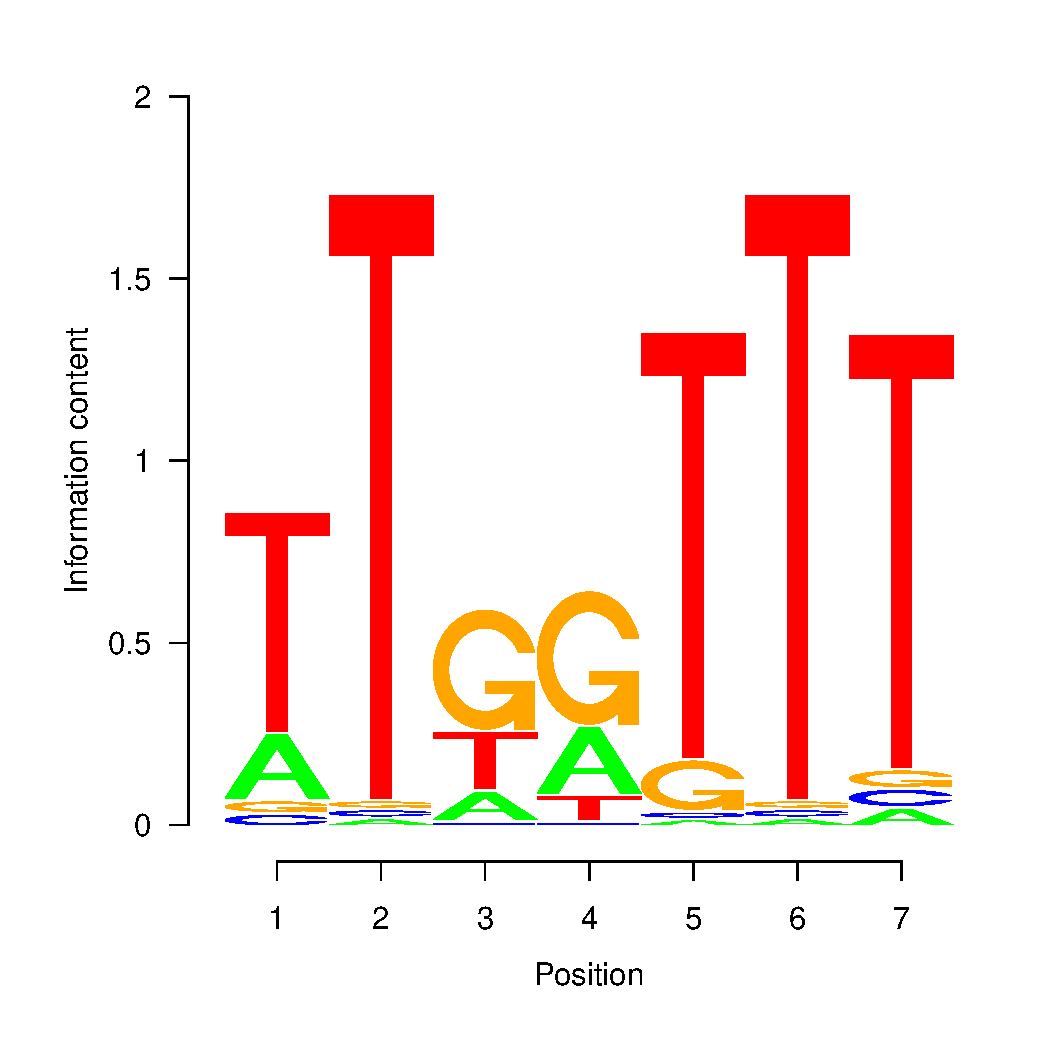
\includegraphics[height=0.8in]{./seqLogo/HuR_uukruuu.pdf} &
 ELAVL1 (aka HuR) is an AU-rich
element (ARE) and U-rich element (URE) RBP that stabilizes
mRNAs and promotes gene expression. Several roles in mediating alternative splicing have been demonstrated~\cite{Izquierdo2008}.\\
\hline
HNRNPA1 & DUAGGGW & 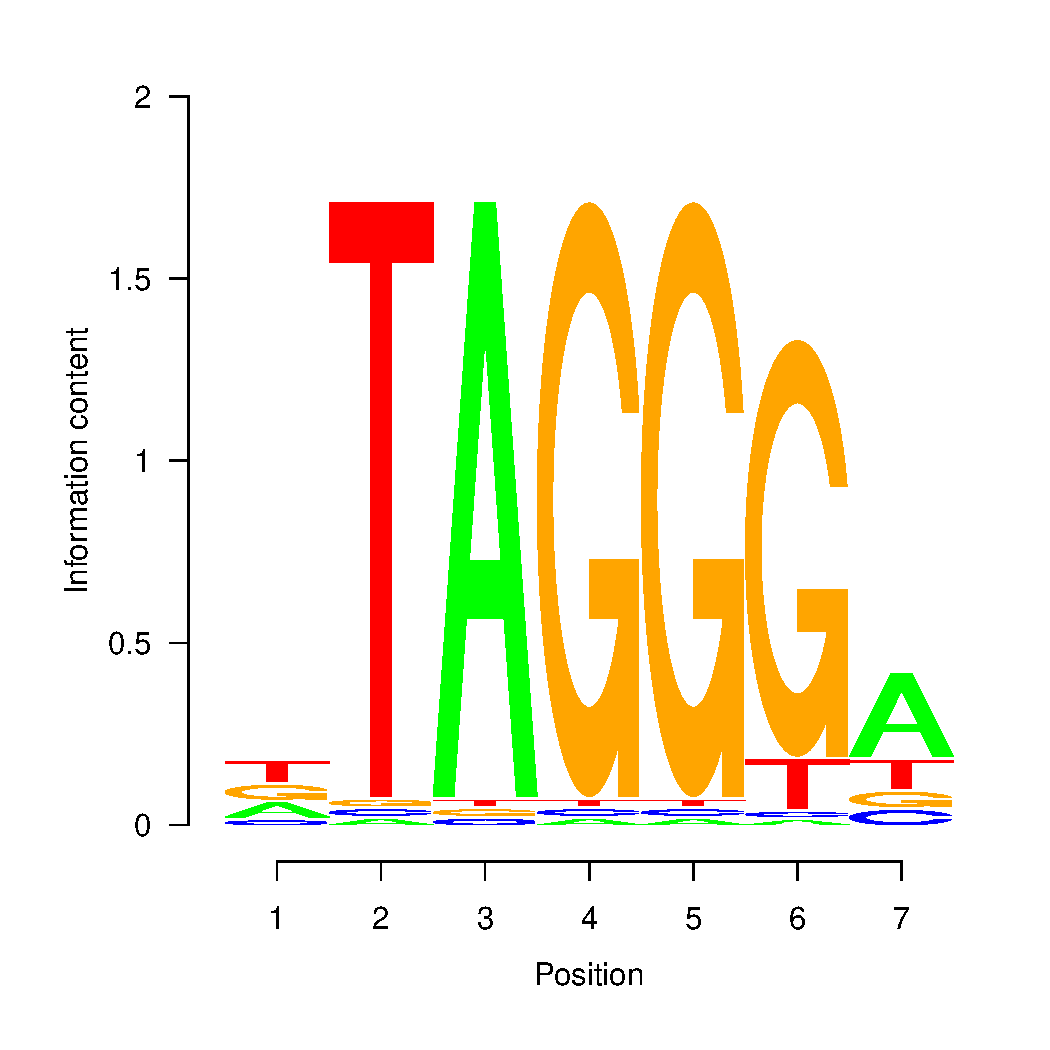
\includegraphics[height=0.8in]{./seqLogo/HNRNPA1_duagggw.pdf}
 & \multirow{22}{6cm}{ 
 \textbf{hnRNPs} \newline
heterogeneous nuclear ribonucleoproteins 
function in RNA splicing, 3’ end processing, trnascriptiona regulation mRNA export, localization, translation and mRNA stability
 function as antagonist to SR in regulating RNA splicing
many hnRNPs share common domain and share function
 Polypyrimide tract binding protein 1(PTB1)
Usually promotes skipping of alternative exon by binding to silence elements
DAZAP1 is a ubiquitous heterogeneous nuclear ribonucleoprotein (hnRNP) that is expressed abundantly in the testis with a role in RNA splicing~\cite{Chen2013}.
FUS is a multifunctional protein component of the heterogeneous nuclear ribonucleoprotein (hnRNP) complex~\cite{Rogelj2012}. RALY, also known as hnRNP
C-related protein, is a member
of the hnRNP family that was initially identified as an
autoantigen cross-reacting with the Epstein−Barr nuclear
antigen 1~\cite{Tenzer2013}.  Transactivation response element DNA-binding protein 43 (TDP-43, TARDBP), is a heterogeneous nuclear ribonucleoprotein (hnRNP)\cite{Ling2015}
 }\\
 \cline{1-3}
HNRNPA1 & GUAGUAGU & 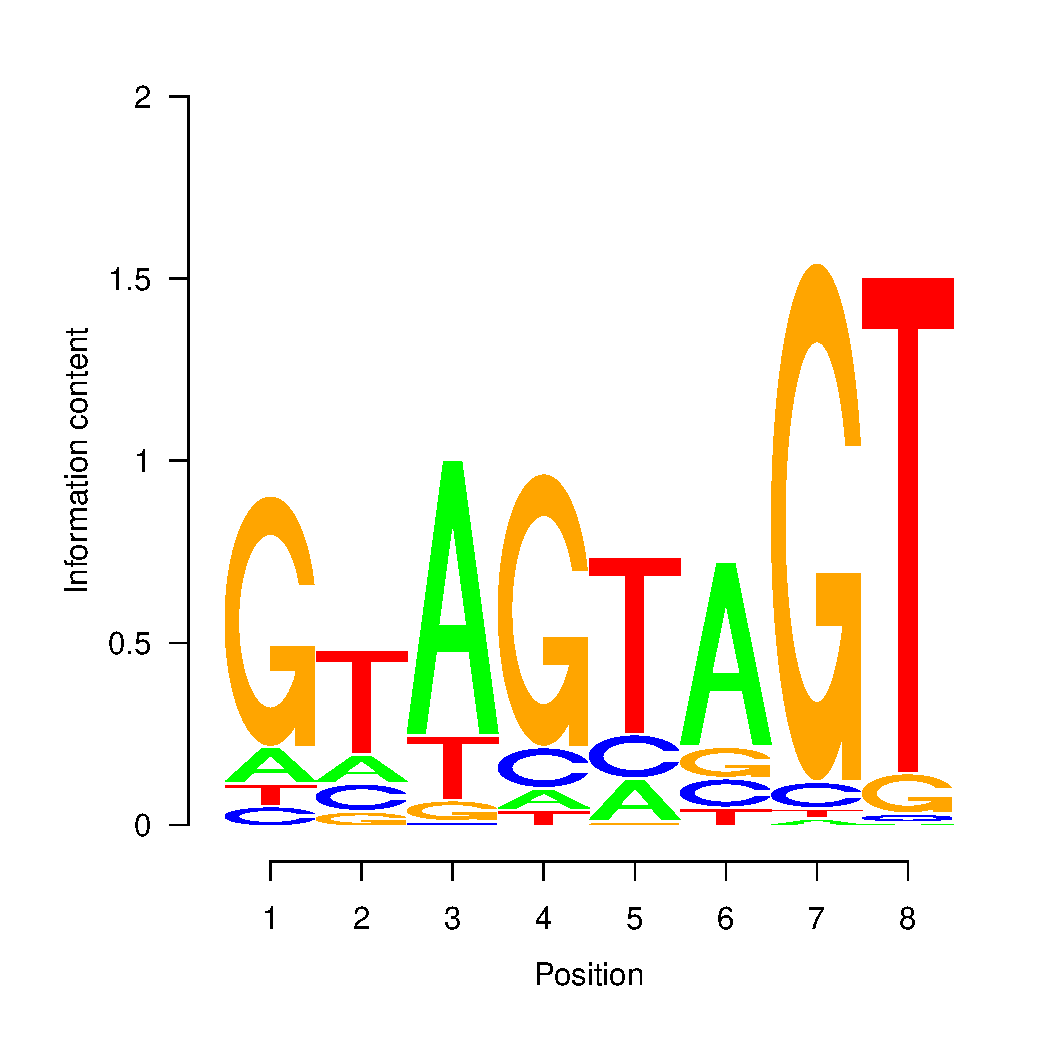
\includegraphics[height=0.8in]{./seqLogo/HNRNPA1_guaguagu.pdf}
 & \\
 \cline{1-3}
HNRNPA1 & RGNYAG & 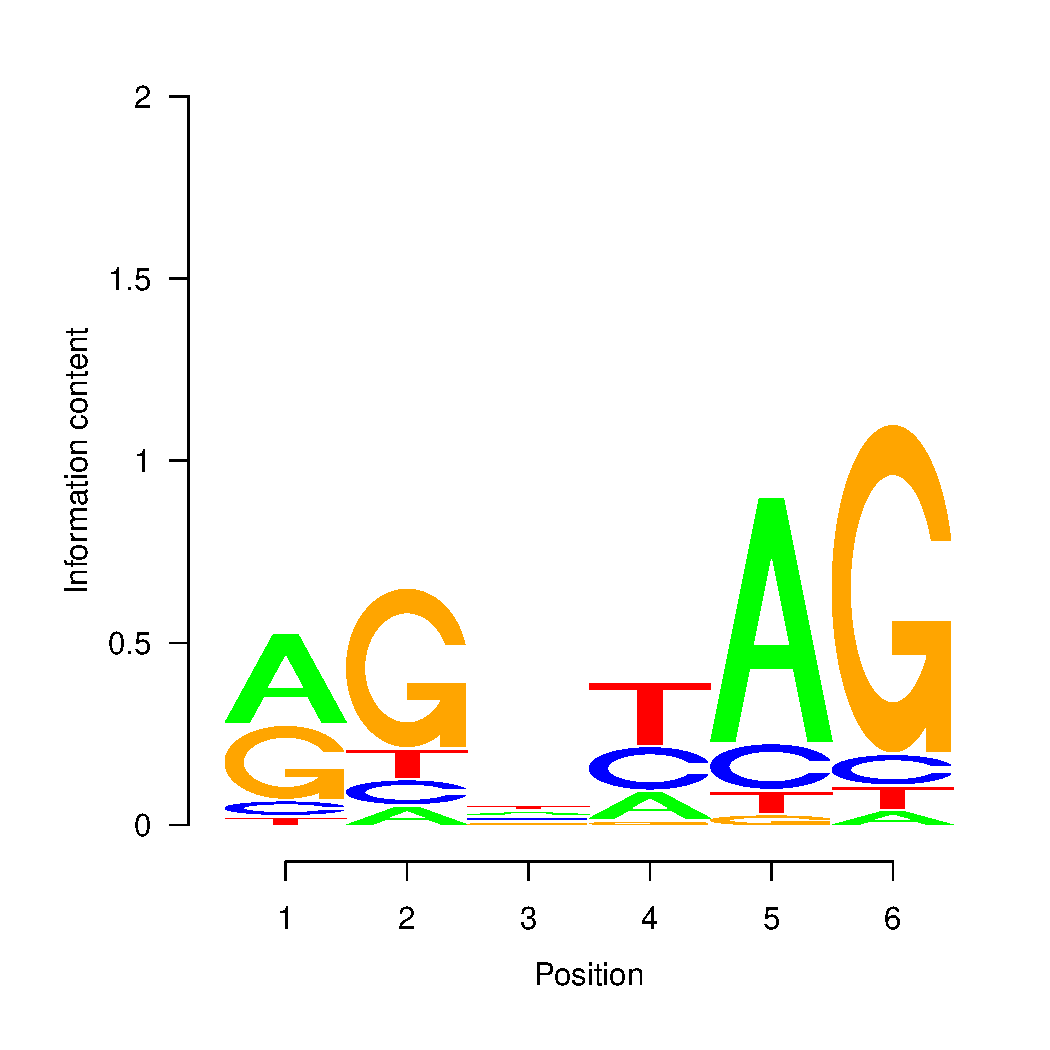
\includegraphics[height=0.8in]{./seqLogo/HNRNPA1_rgnyag.pdf}
 &  \\
 \cline{1-3}
 HNRNPA1L2 & DUAGGGW &  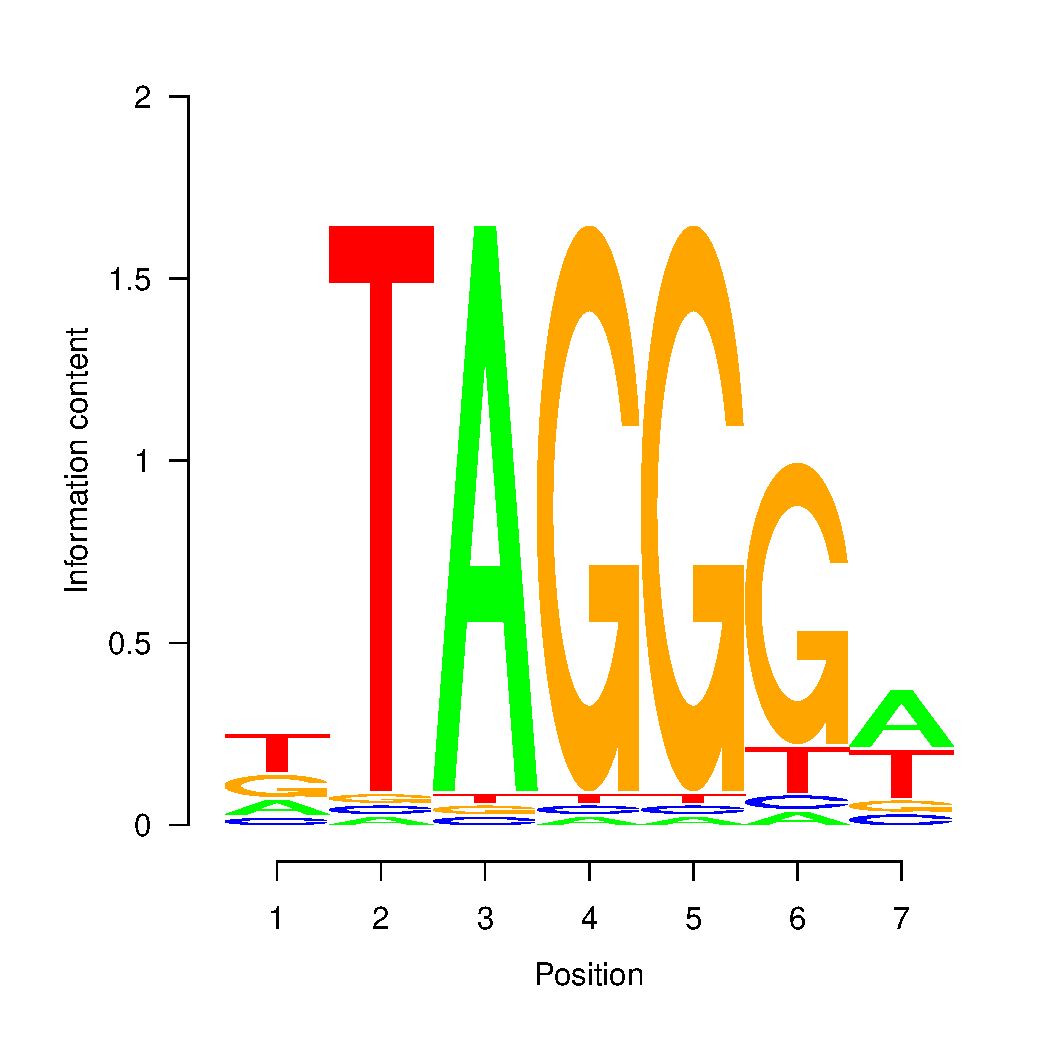
\includegraphics[height=0.8in]{./seqLogo/HNRNPA1L2_duagggw.pdf}
&  \\
\cline{1-3}
HNRNPA2B1 & AGGWUHGR &  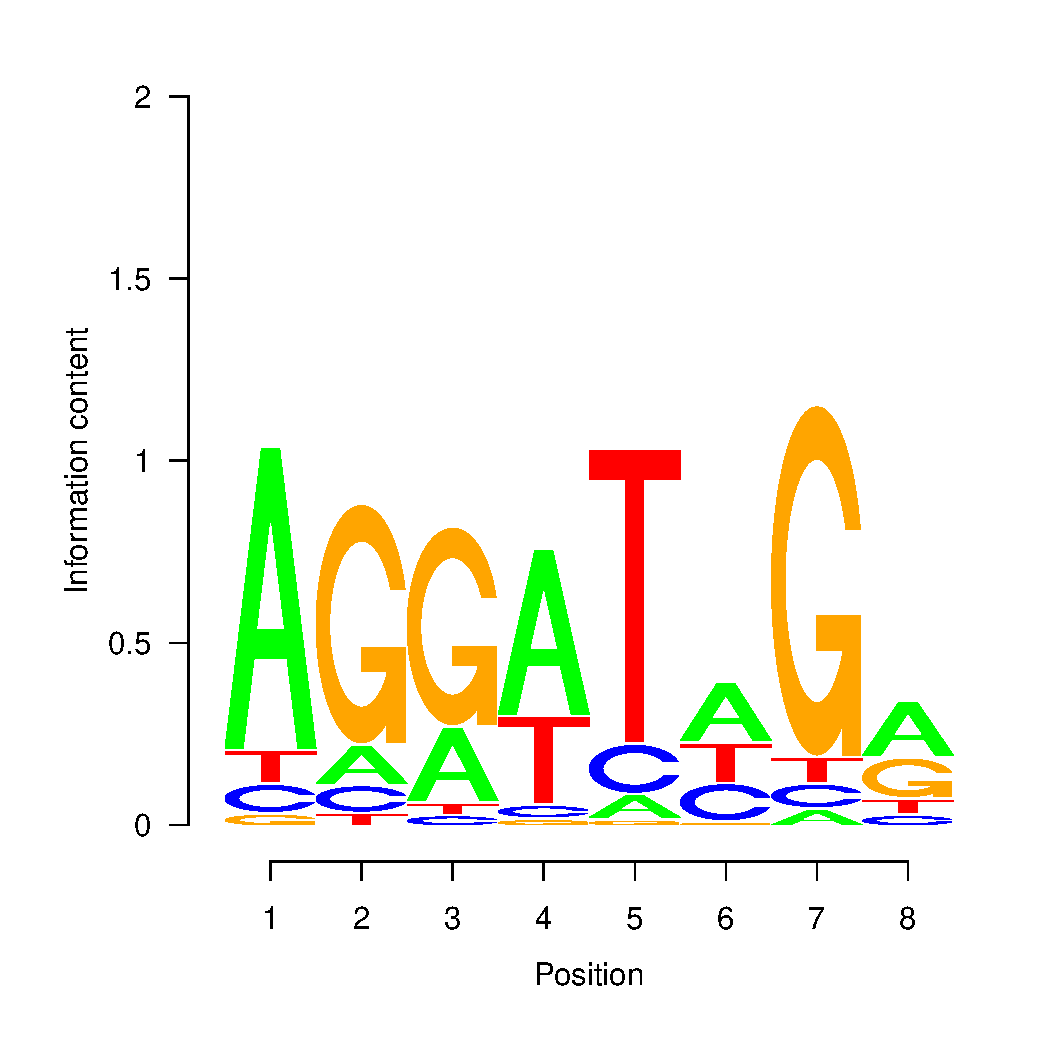
\includegraphics[height=0.8in]{./seqLogo/HNRNPA2B1_aggwuhgr.pdf}
 &  \\
 \cline{1-3}
HNRNPA2B1 & DUAGGGW &  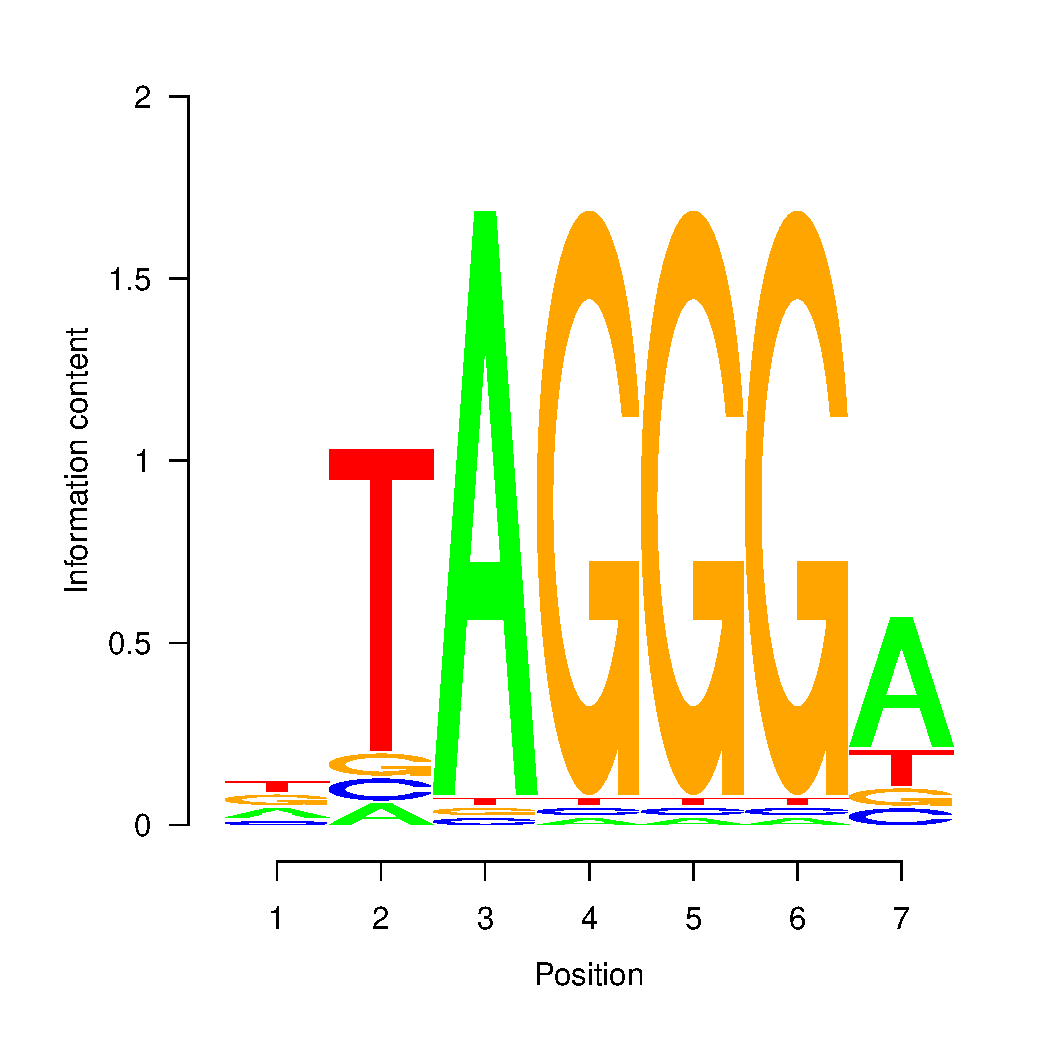
\includegraphics[height=0.8in]{./seqLogo/HNRNPA2B1_duagggw.pdf}
 & \\
 \cline{1-3}
HNRNPA2B1 & GGUAGUAG &  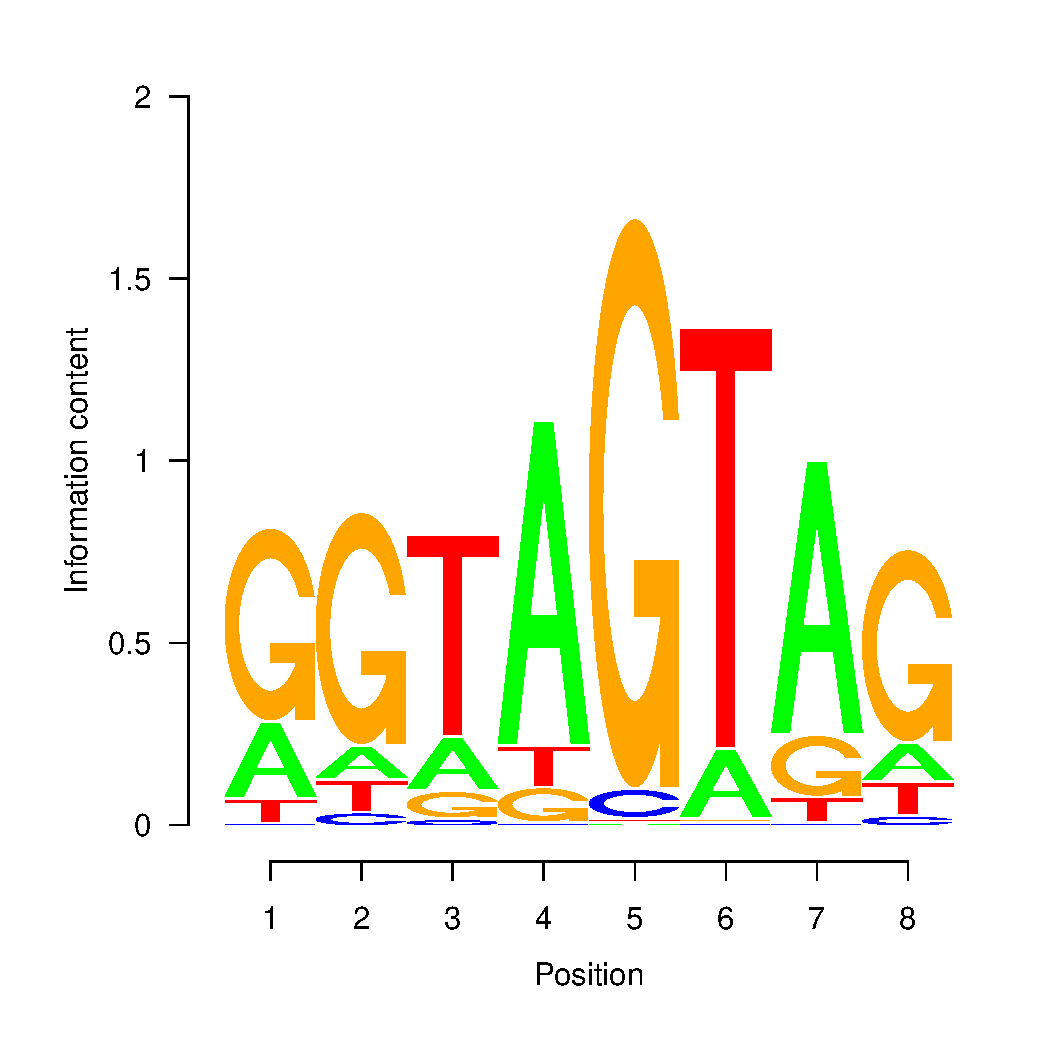
\includegraphics[height=0.8in]{./seqLogo/HNRNPA2B1_gguaguag.pdf}
 &  \\
 \cline{1-3}
HNRNPC &  HUUUUUK & 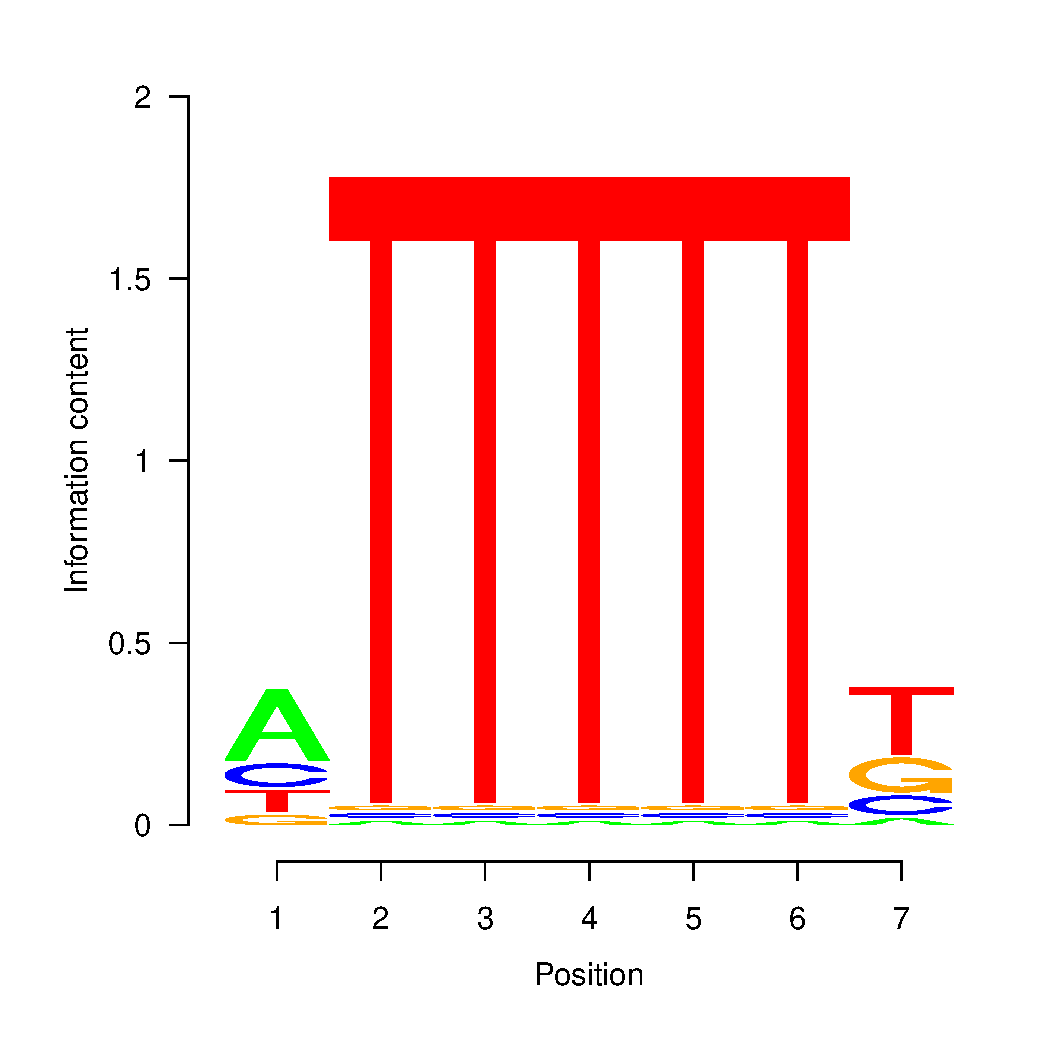
\includegraphics[height=0.8in]{./seqLogo/HNRNPC_huuuuuk.pdf}
 &  \\
 \cline{1-3}
HNRNPCL1 & HUUUUUK & 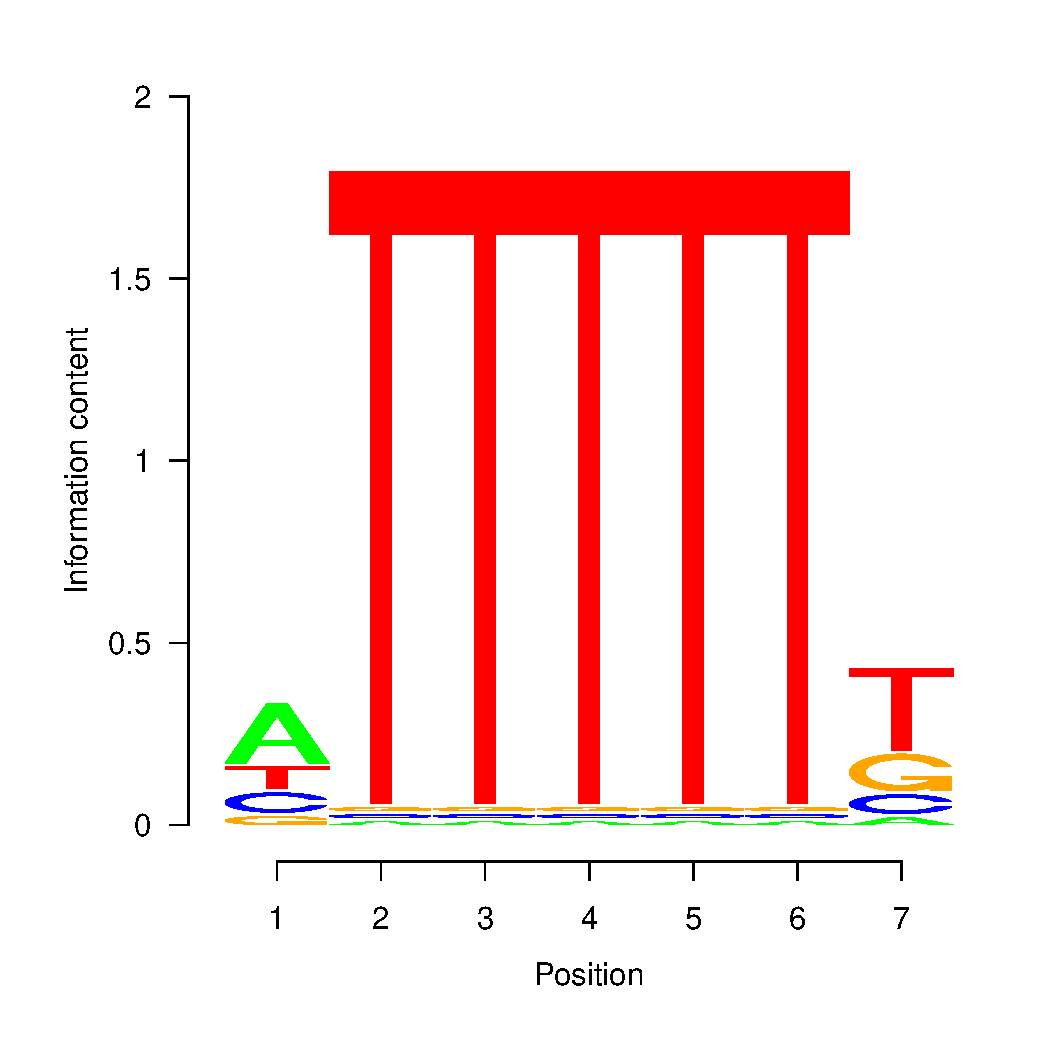
\includegraphics[height=0.8in]{./seqLogo/HNRNPCL1_huuuuuk.pdf}
 &  \\
 \cline{1-3}
HNRNPF &  GUGKAU & 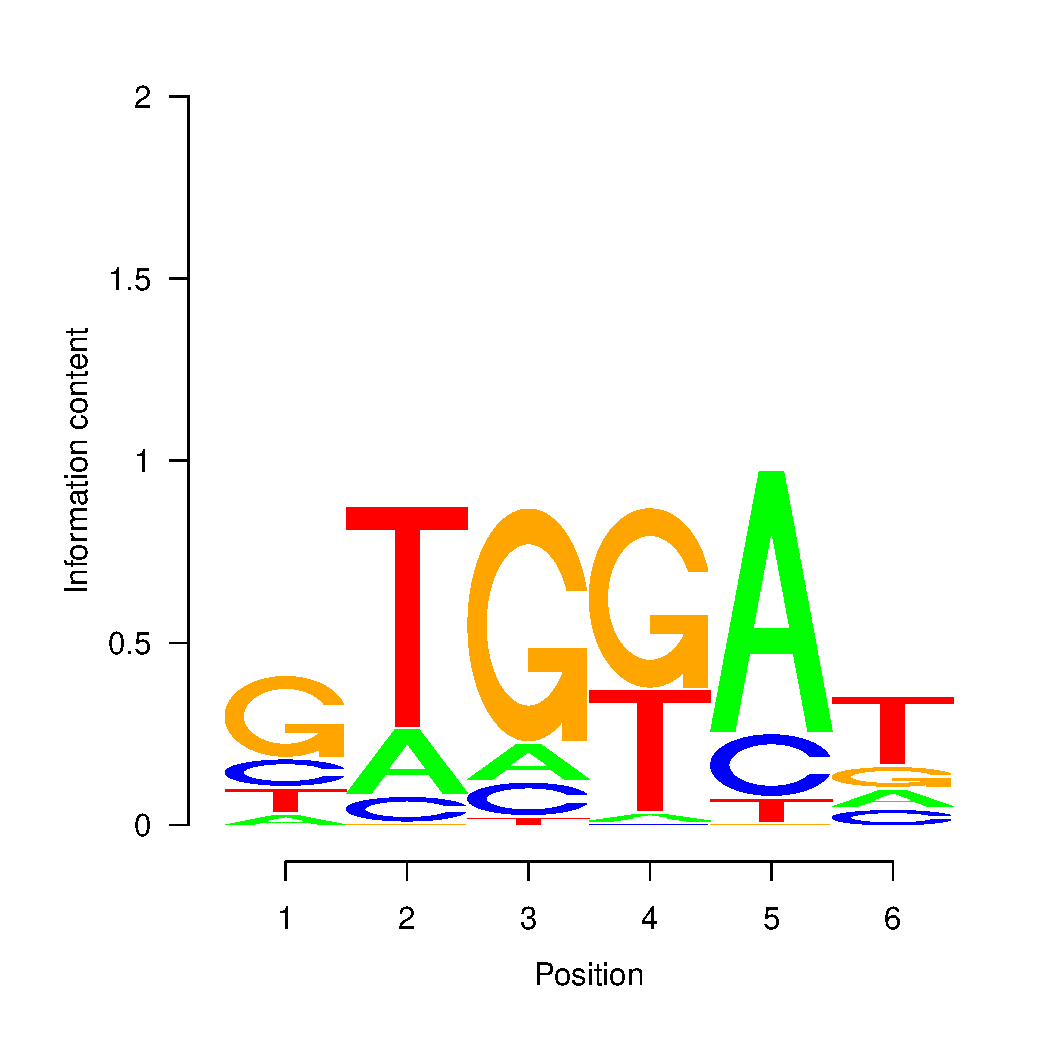
\includegraphics[height=0.8in]{./seqLogo/HNRNPF_gugkau.pdf}
 &  \\
 \cline{1-3}
HNRNPH1 & GARGAG&  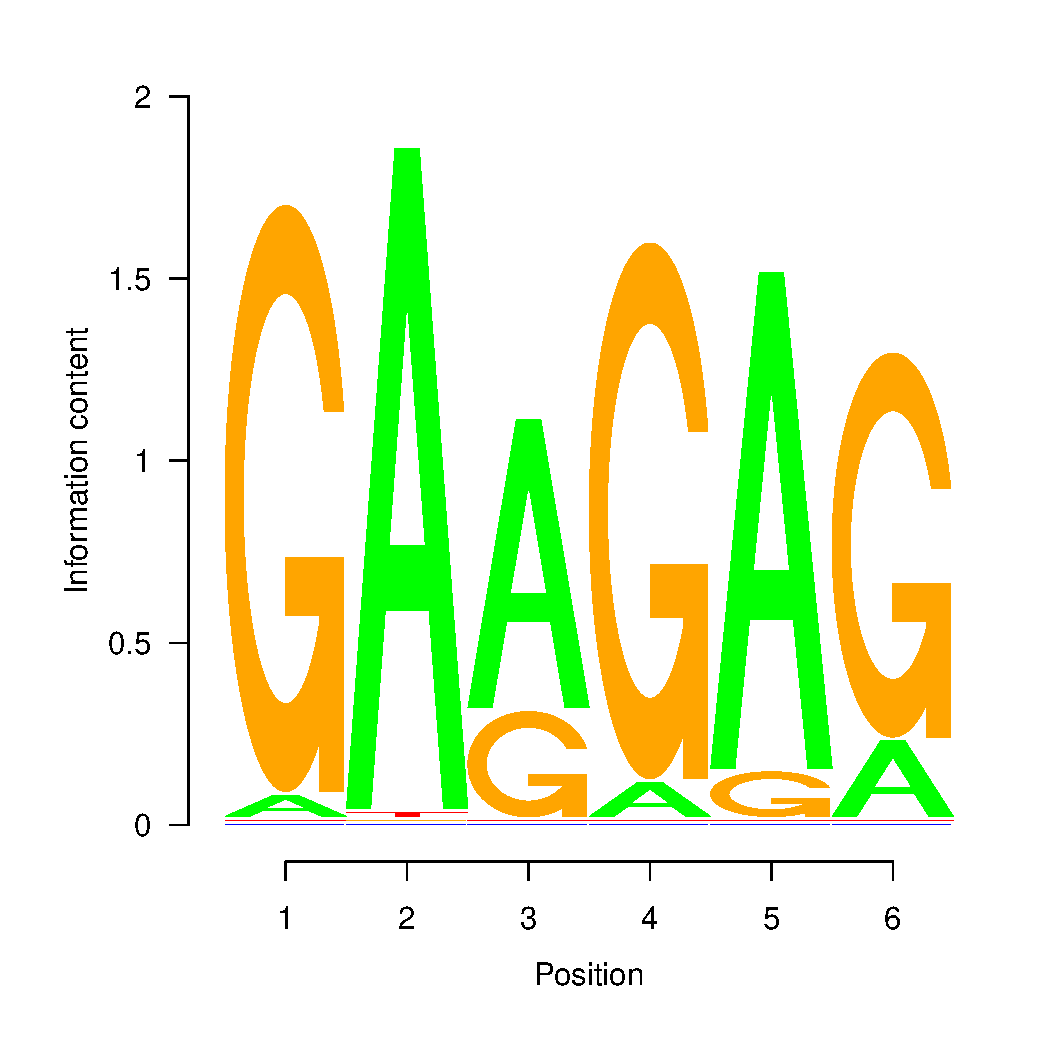
\includegraphics[height=0.8in]{./seqLogo/HNRNPH1_gargag.pdf}
 & \\
 \cline{1-3}
HNRNPH2 &  GGGAGGG & 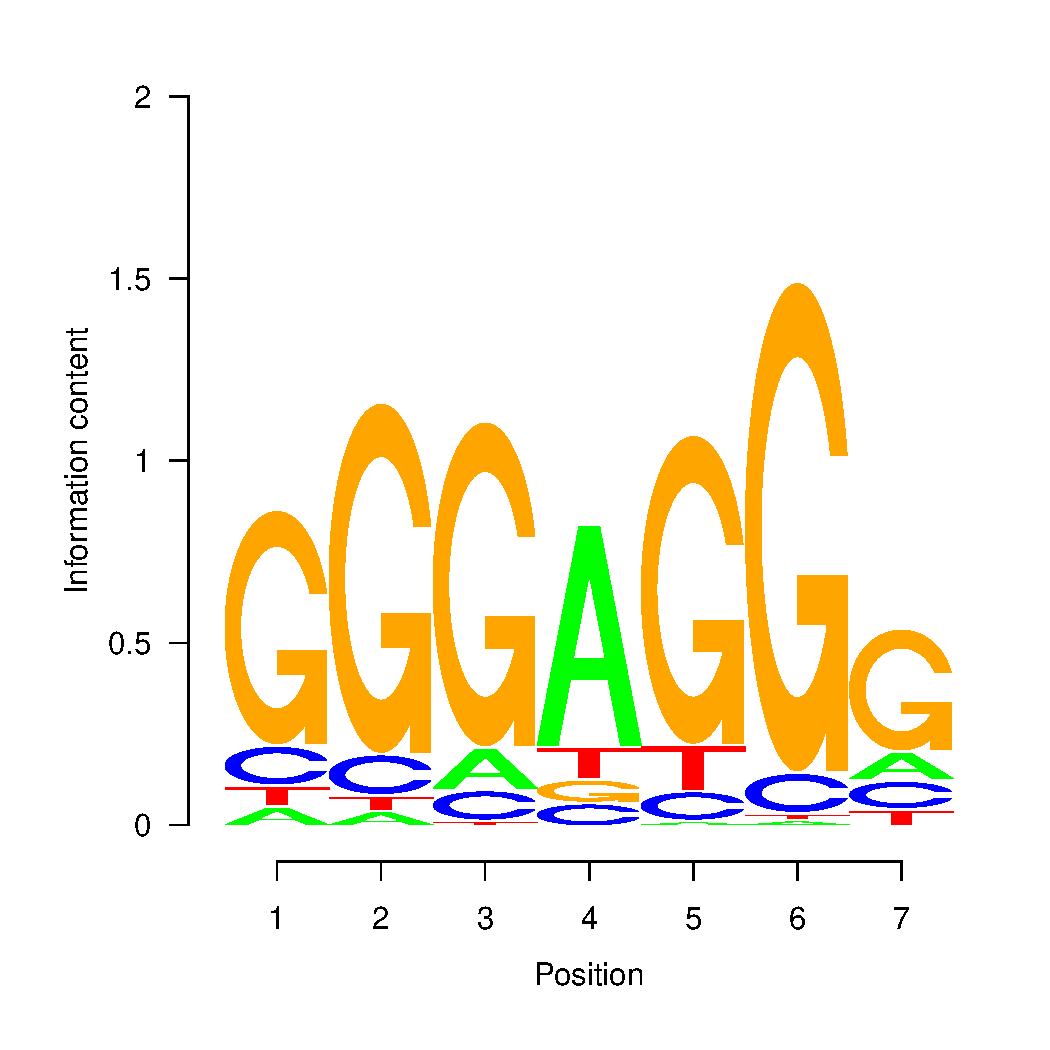
\includegraphics[height=0.8in]{./seqLogo/HNRNPH2_gggaggg.pdf}
 &  \\
 \cline{1-3}
HNRNPK & CCAWMCC &  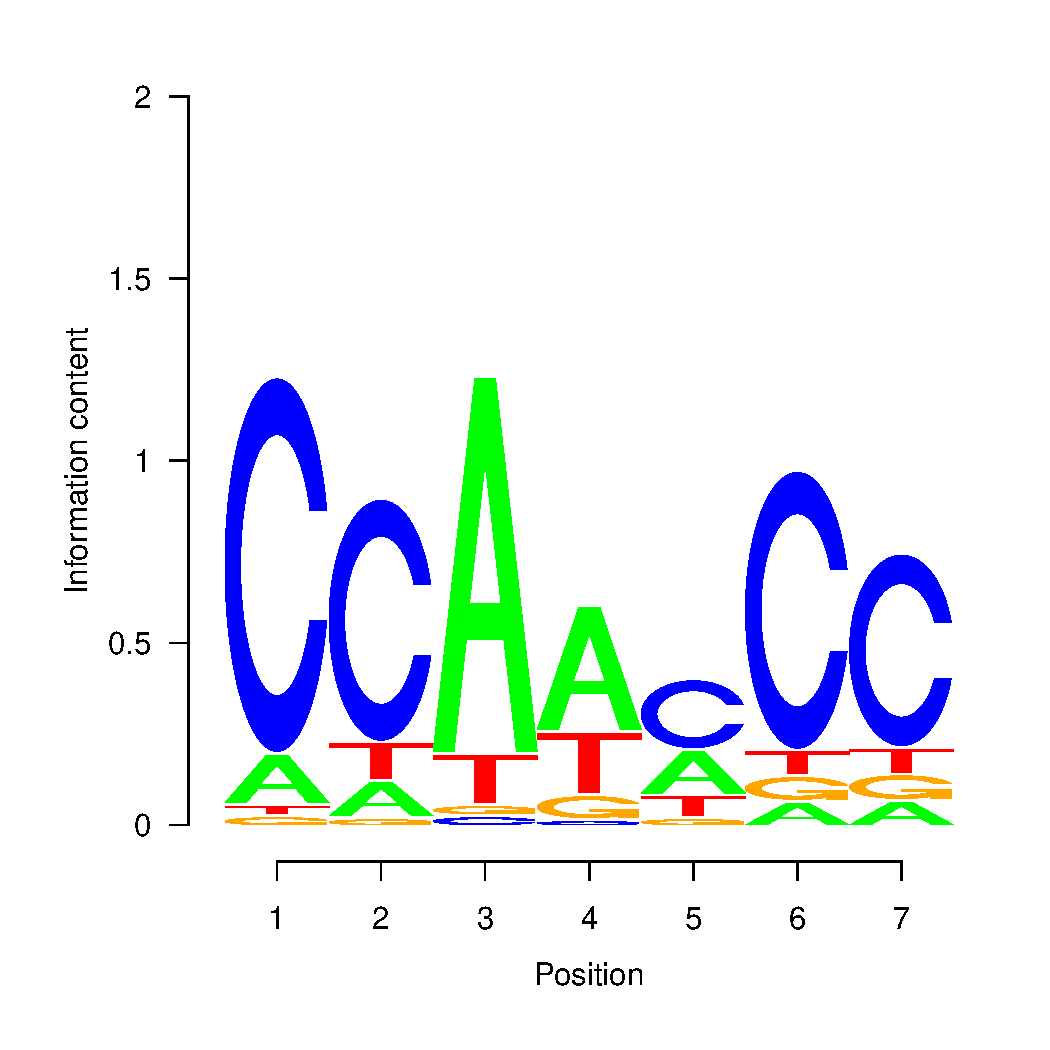
\includegraphics[height=0.8in]{./seqLogo/HNRNPK_ccawmcc.pdf}
 &  \\
 \cline{1-3}
HNRNPL & ACACRAV &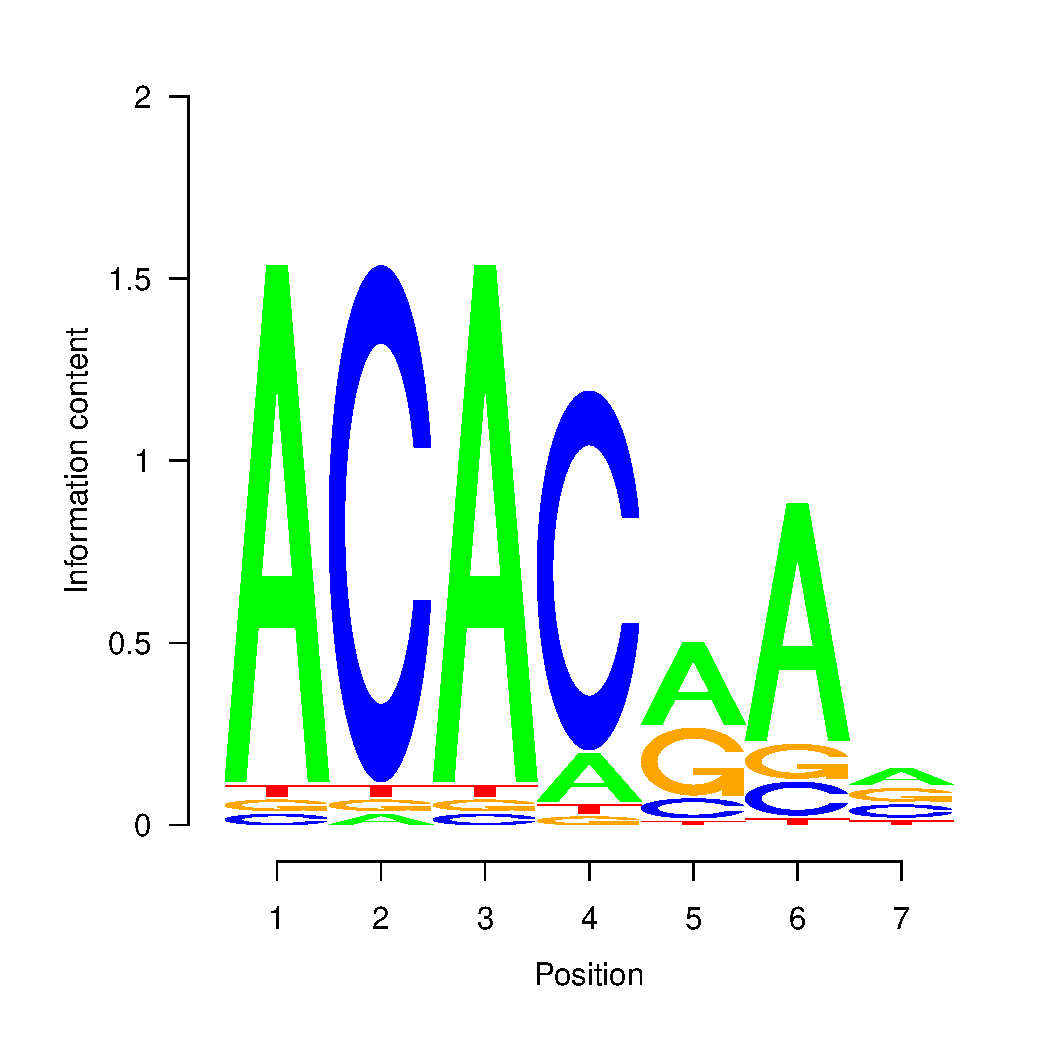
\includegraphics[height=0.8in]{./seqLogo/HNRNPL_acacrav.pdf}
   & \\
\cline{1-3}
HNRNPL & AMAYAMA & 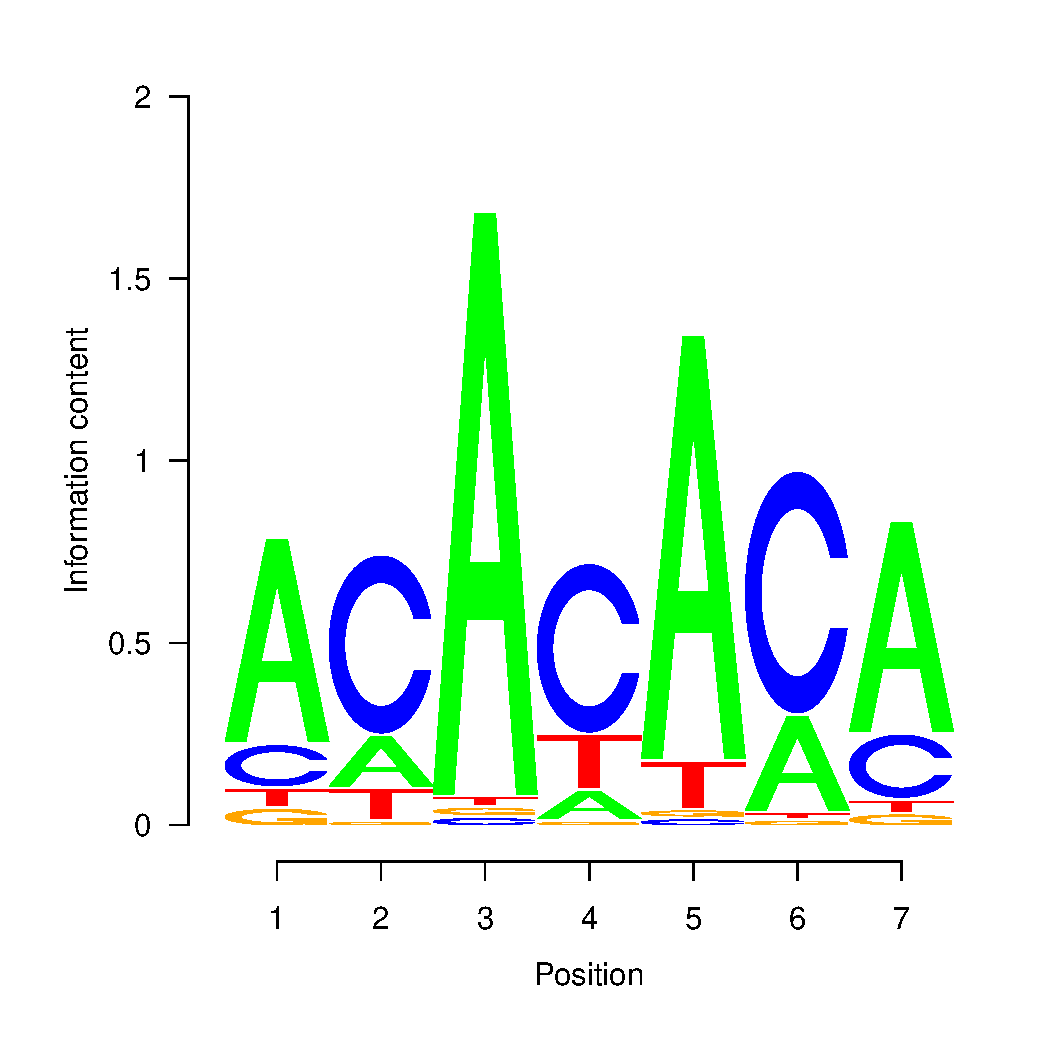
\includegraphics[height=0.8in]{./seqLogo/HNRNPL_amayama.pdf}
 & \\
 \cline{1-3}
HNRNPM & GGUUGGUU &  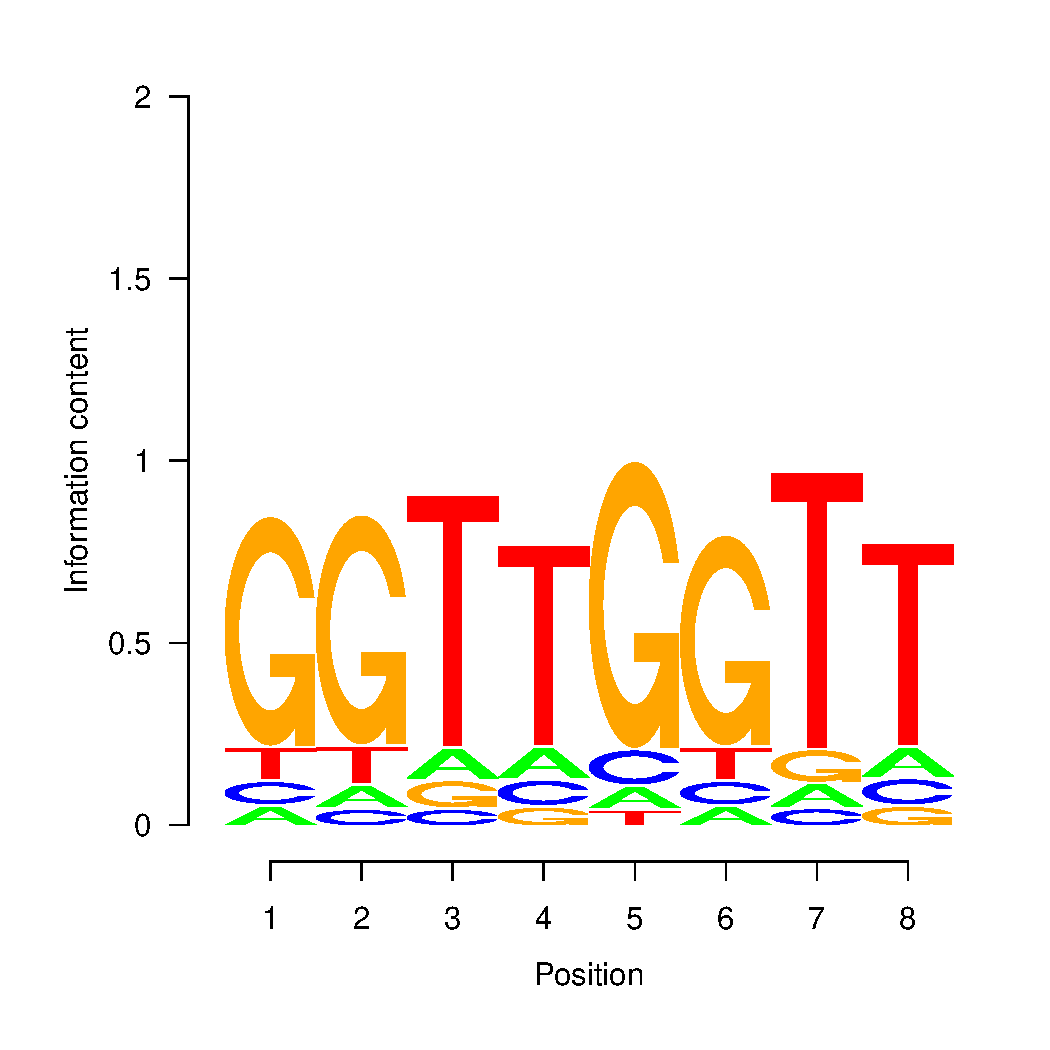
\includegraphics[height=0.8in]{./seqLogo/HNRNPM_gguugguu.pdf}
 & \\
 \cline{1-3}
HNRNPU & UGUAUUG & 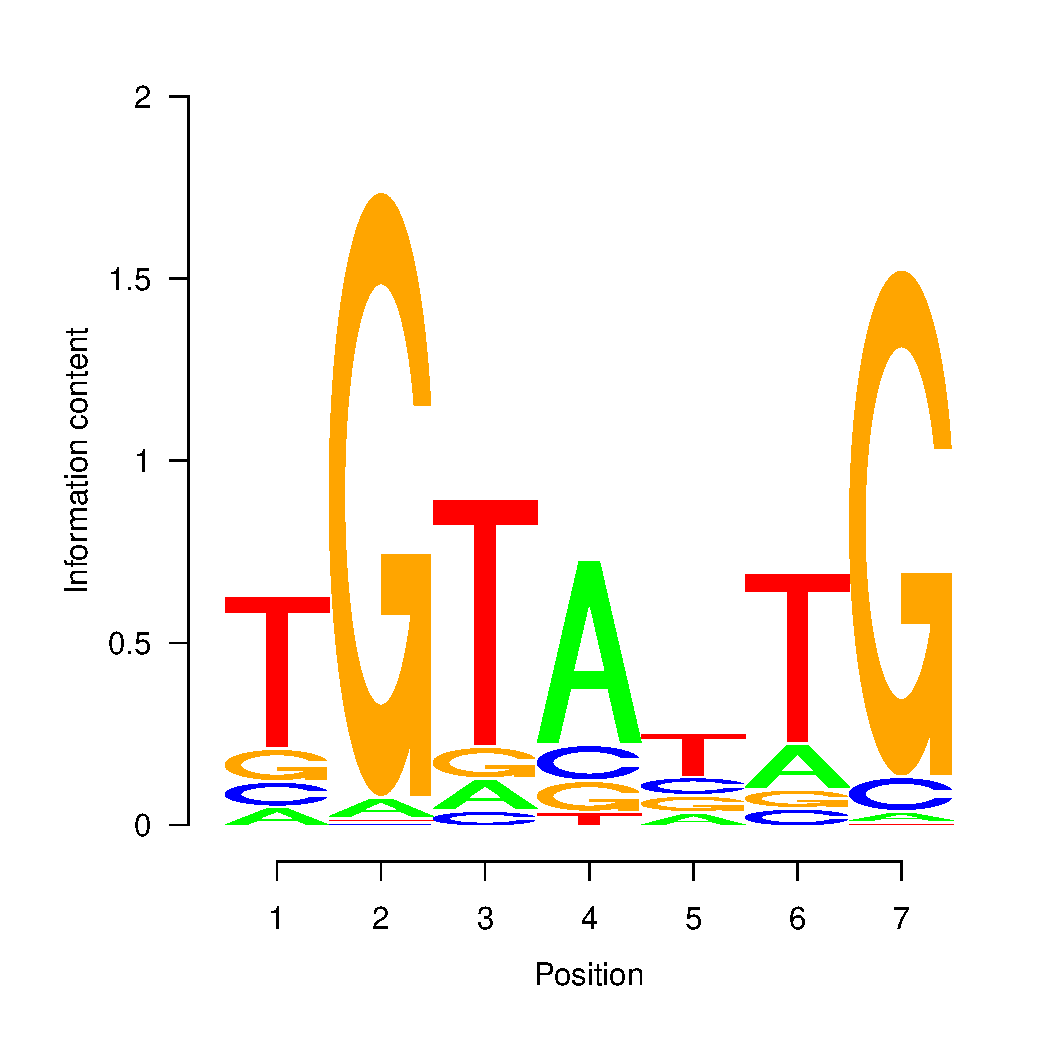
\includegraphics[height=0.8in]{./seqLogo/HNRNPU_uguauug.pdf}
 &  \\
 \cline{1-3}
HNRPLL & RCAHACA & 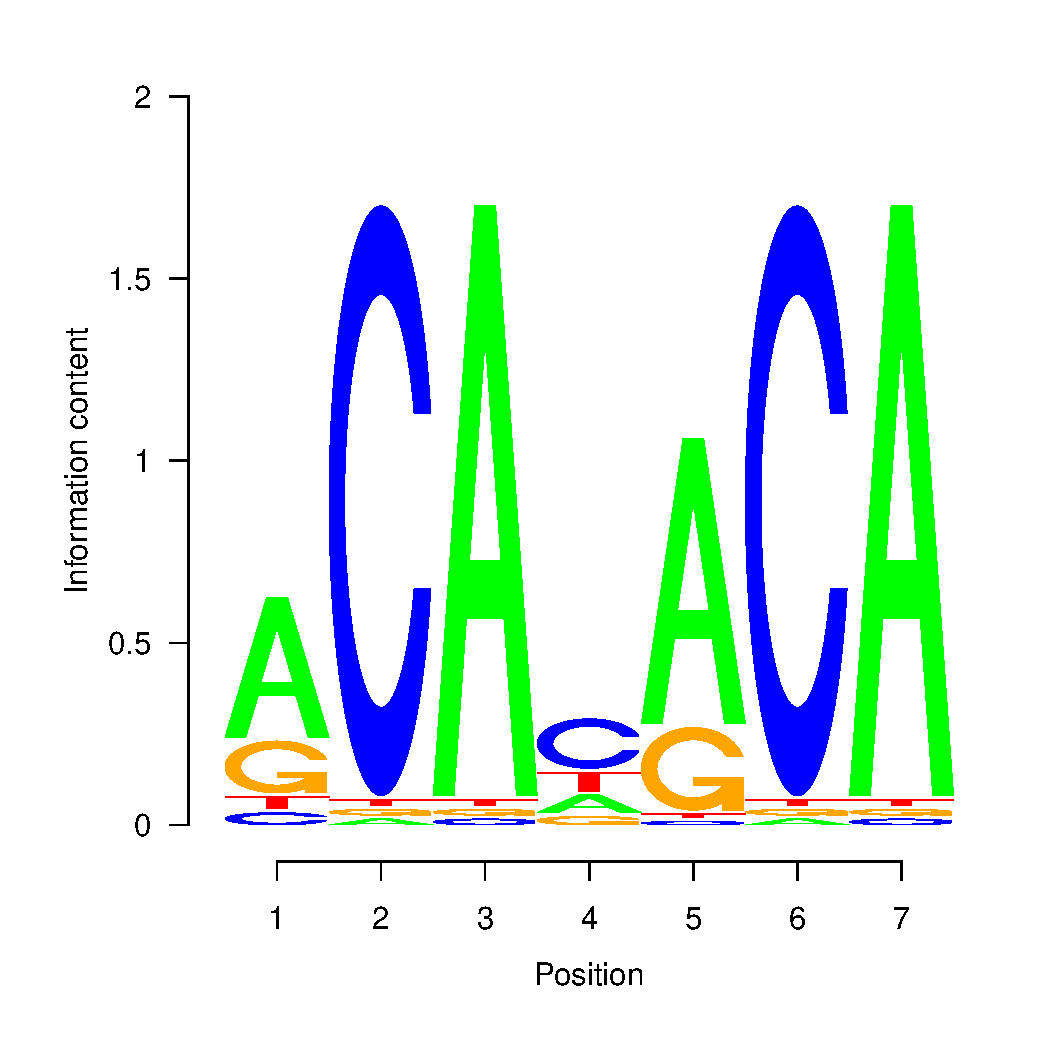
\includegraphics[height=0.8in]{./seqLogo/HNRPLL_rcahaca.pdf}
 & \\
 \cline{1-3}
PTBP1 &  HYUUUYU & 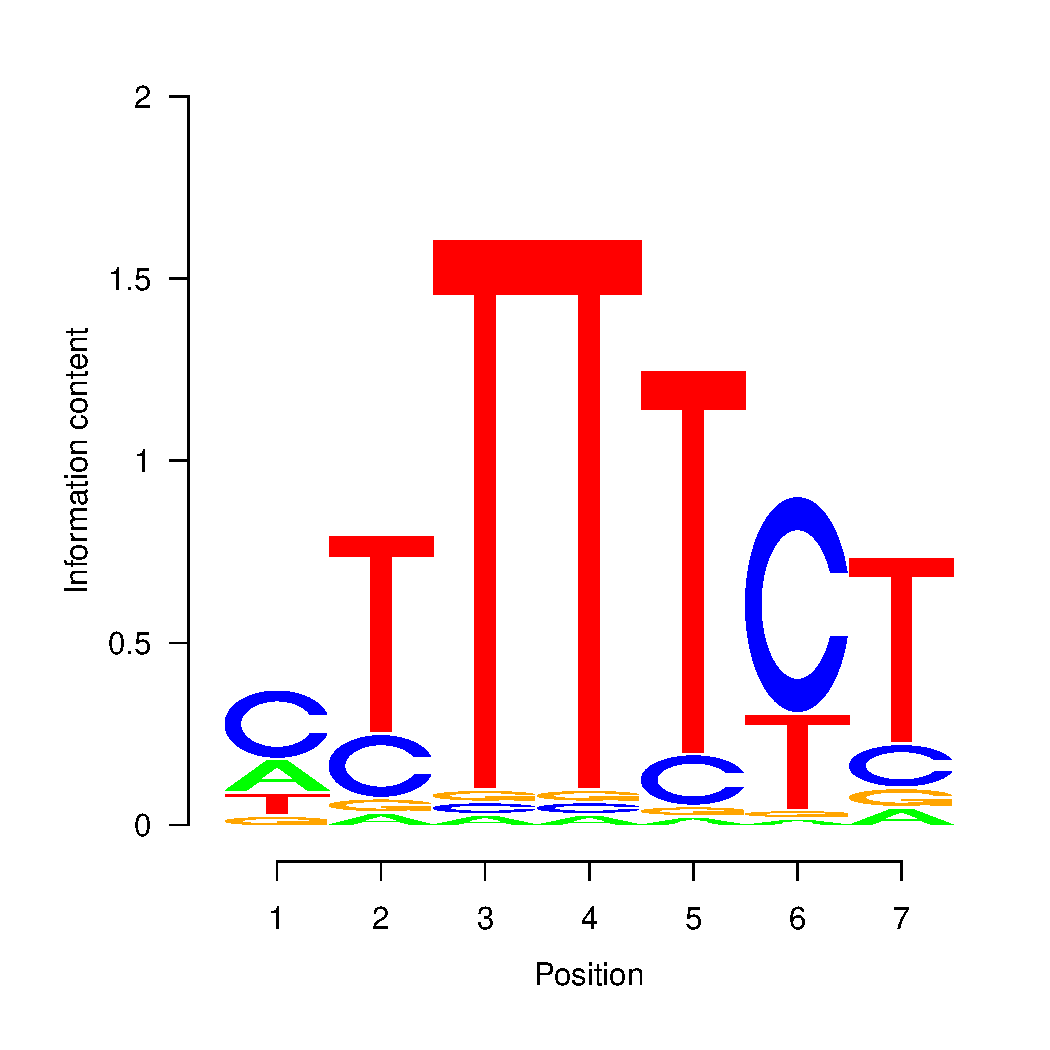
\includegraphics[height=0.8in]{./seqLogo/PTBP1_hyuuuyu.pdf}
 &  \\
  \cline{1-3}
 DAZAP1 & UAGKWWR &  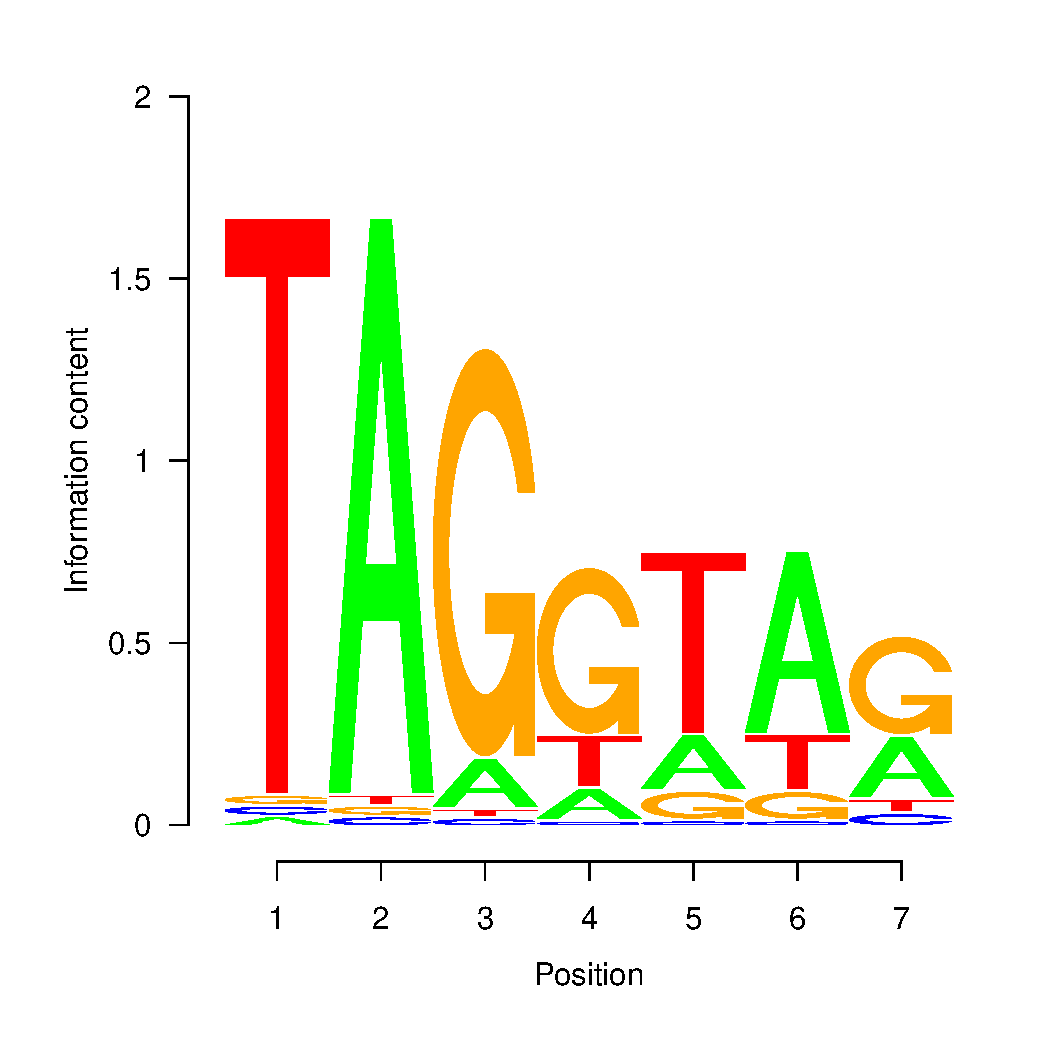
\includegraphics[height=0.8in]{./seqLogo/DAZAP1_uagkwwr.pdf} & \\
  \cline{1-3}
FUS & CGCGC & 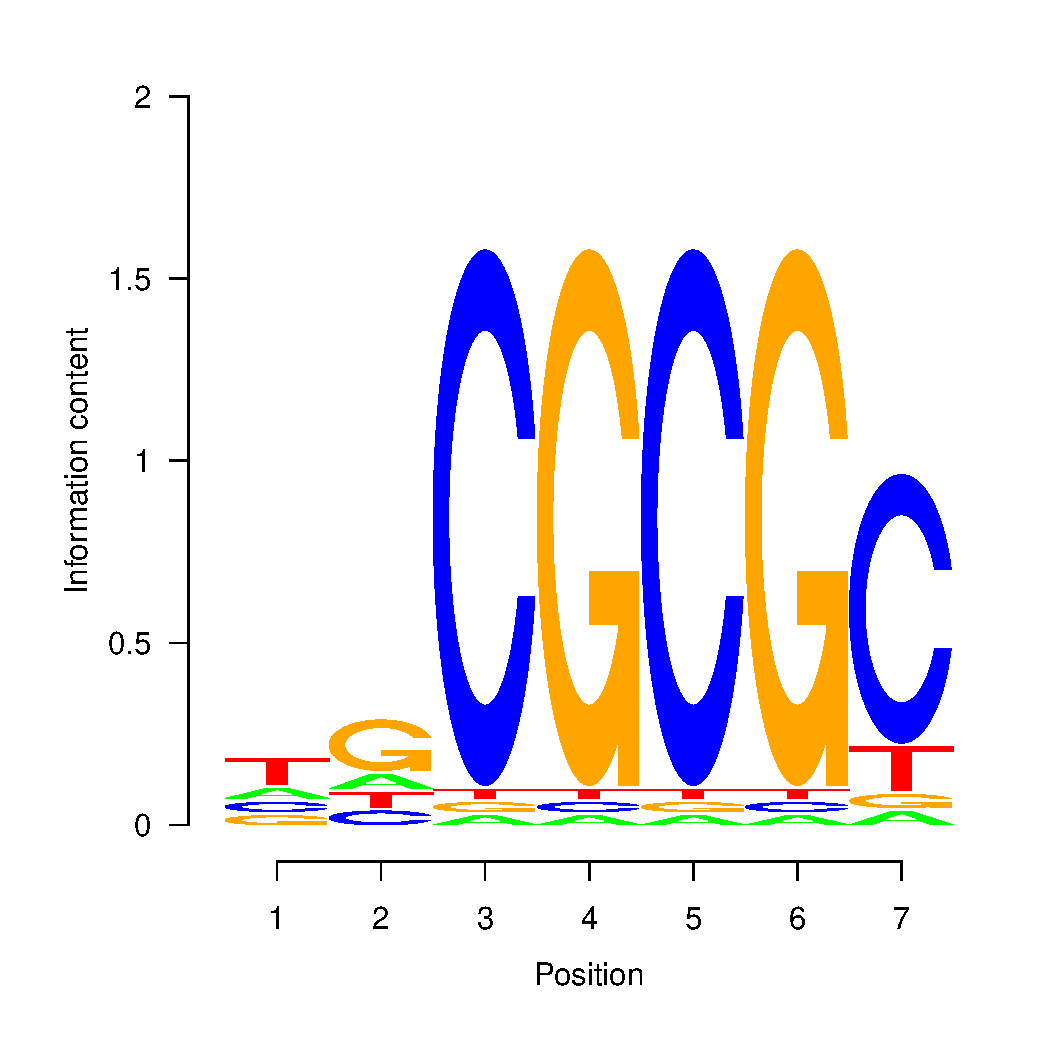
\includegraphics[height=0.8in]{./seqLogo/FUS_cgcgc.pdf} & \\
\cline{1-3}
RALY & & 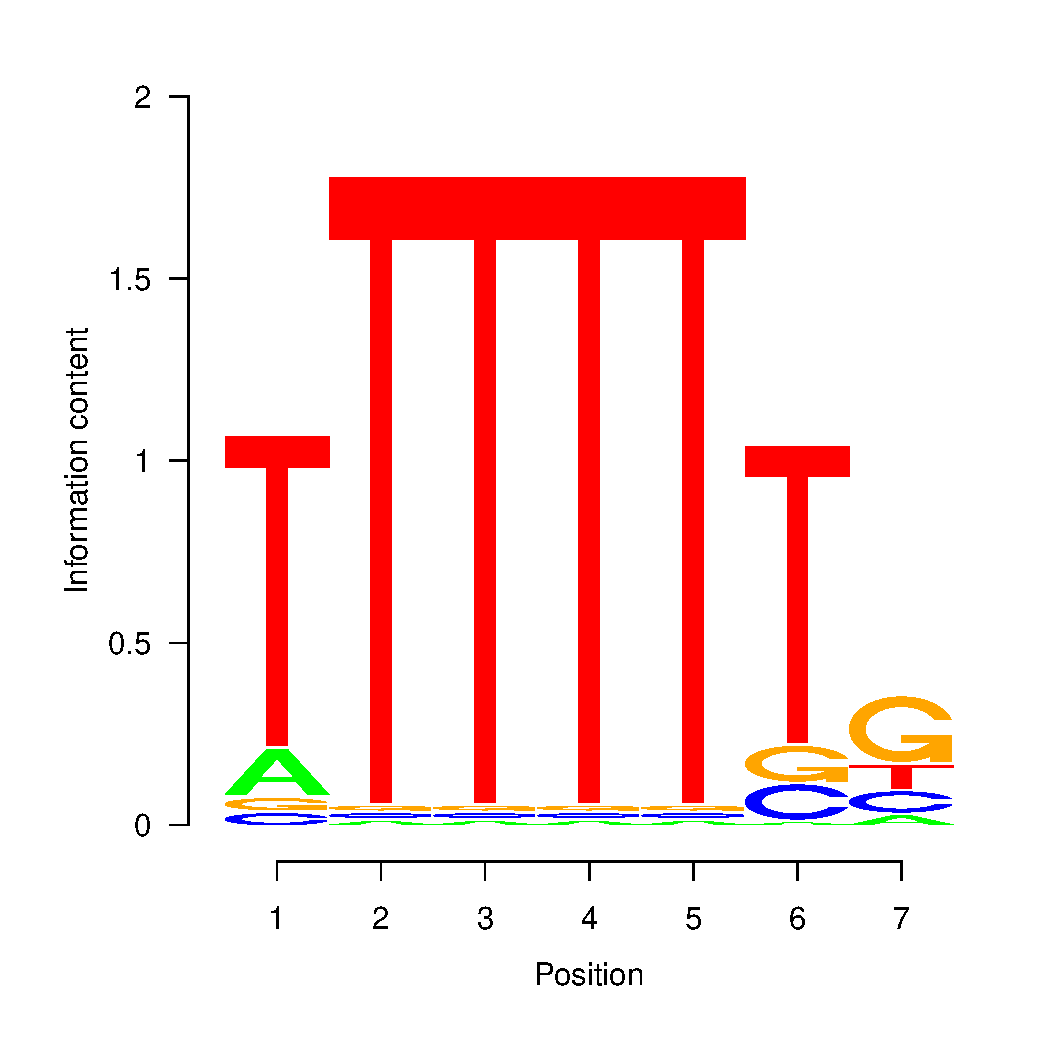
\includegraphics[height=0.8in]{./seqLogo/RALY_uuuuuub.pdf} & \\
\cline{1-3}
TARDBP & GAAUGD  & 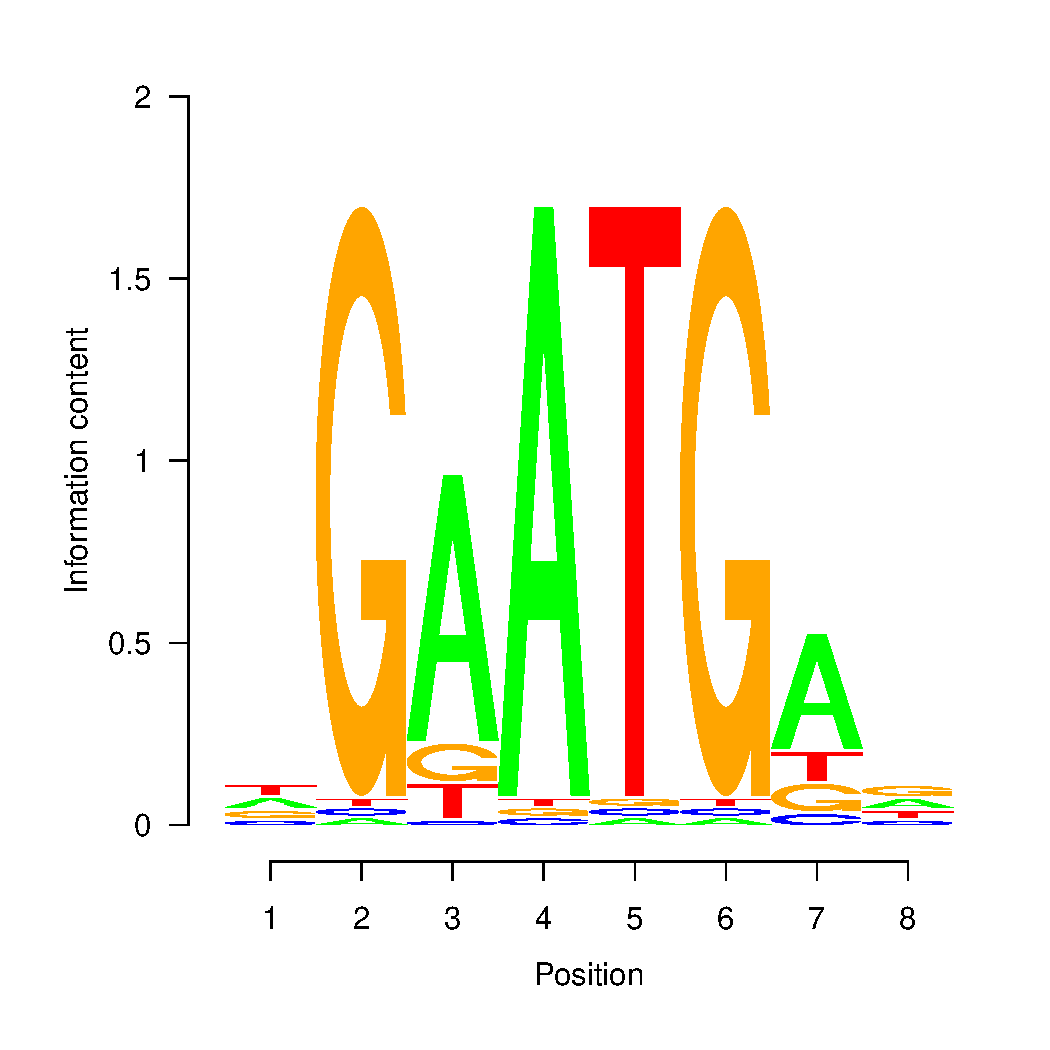
\includegraphics[height=0.8in]{./seqLogo/TARDBP_gaaugd.pdf} & \\
\hline
RBFOX1 & WGCAUGM & 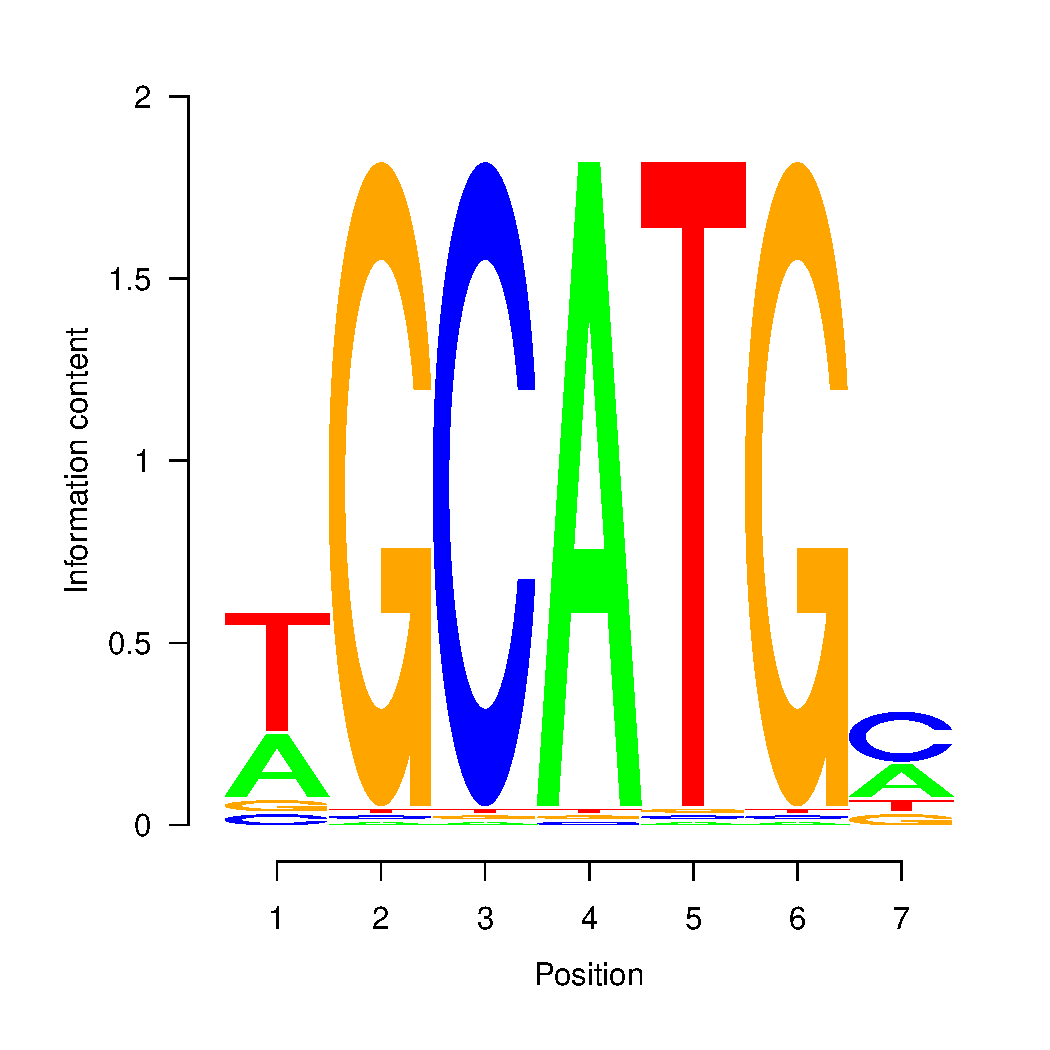
\includegraphics[height=0.8in]{./seqLogo/RBFOX1_wgcaugm.pdf}
 & Function in splicing activation and repression
Modulate splicing outcomes in position-specific manner. Rbfox upstream of an exon suppresses and binding downstream of an exon enhances exon inclusion.
 \\
CELF4 & KGUGUKK & 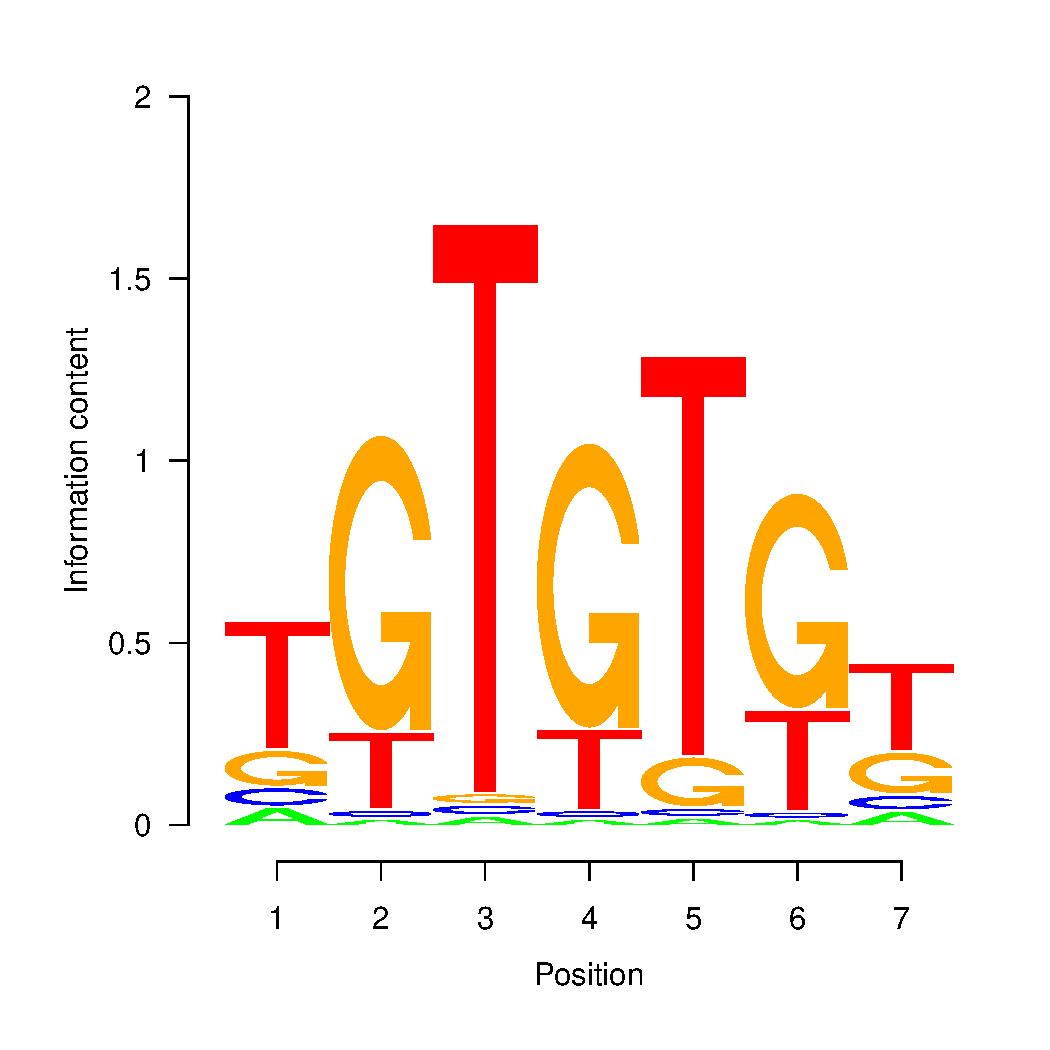
\includegraphics[height=0.8in]{./seqLogo/BRUNOL4_kgugukk.pdf} 
 & \multirow{3}{6cm}{ 
 \textbf{CELF/BRUNOL family} \newline
Members of the CELF/BRUNOL protein family, which are characterized by two N-terminal RNA recognition motif (RRM) domains and one C-terminal RRM domains, regulate pre-mRNA alternative splicing and may also be involved in mRNA editing, and translation~\cite{Wagnon2012}.\\
}\\
CELF5 & UGUGUKK & 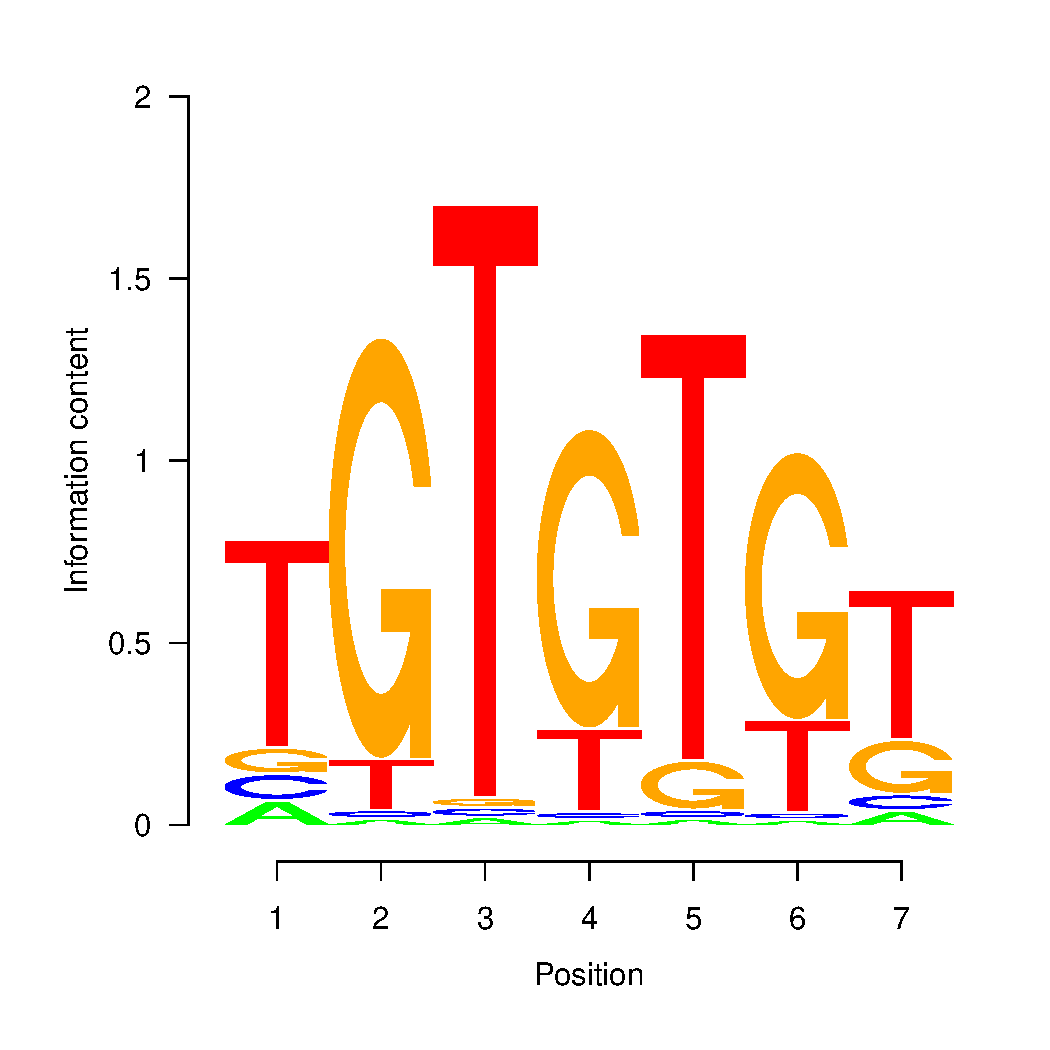
\includegraphics[height=0.8in]{./seqLogo/BRUNOL5_ugugukk.pdf} & \\
CELF6 & UGUGDKG & 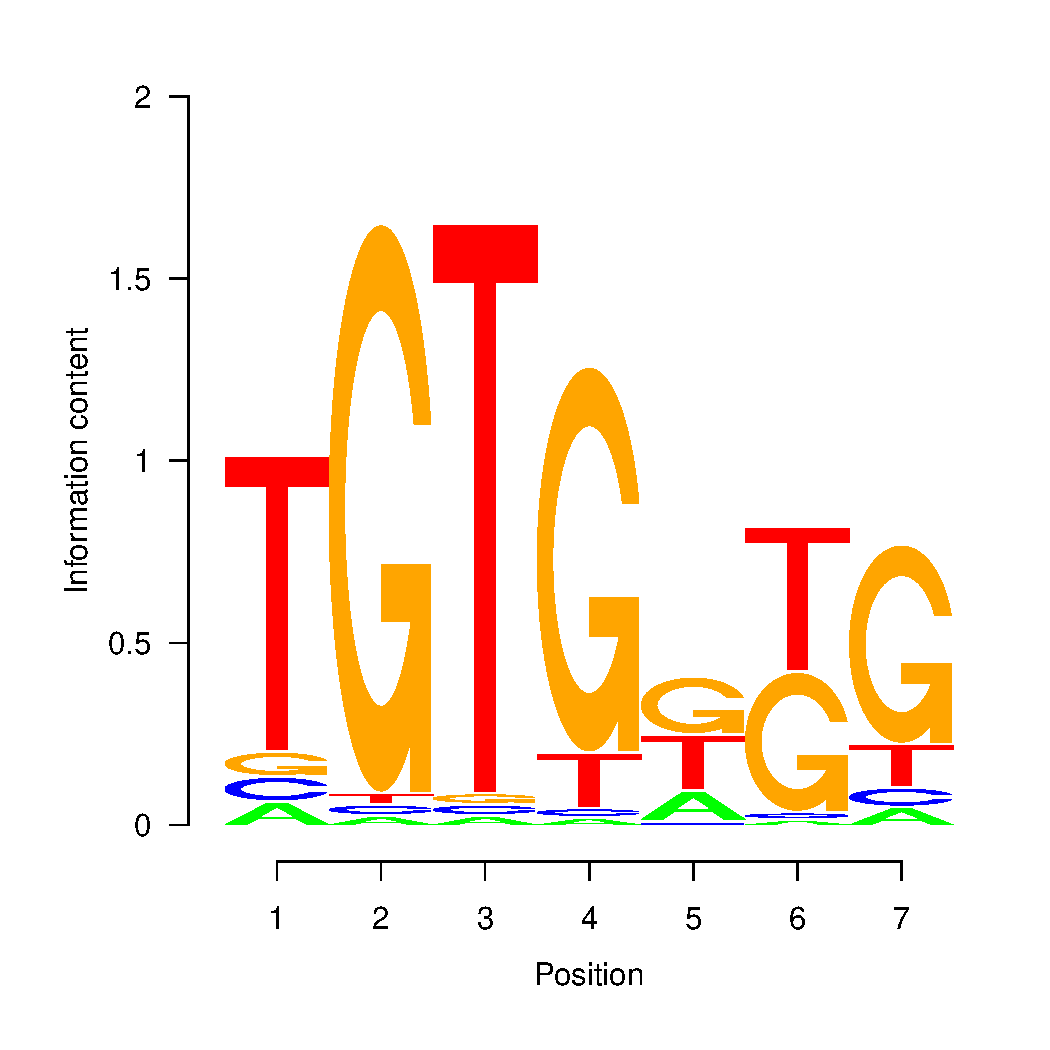
\includegraphics[height=0.8in]{./seqLogo/BRUNOL6_ugugdkg.pdf}& \\
  \hline

 \hline
 ESPR2 & UGGGRAD &  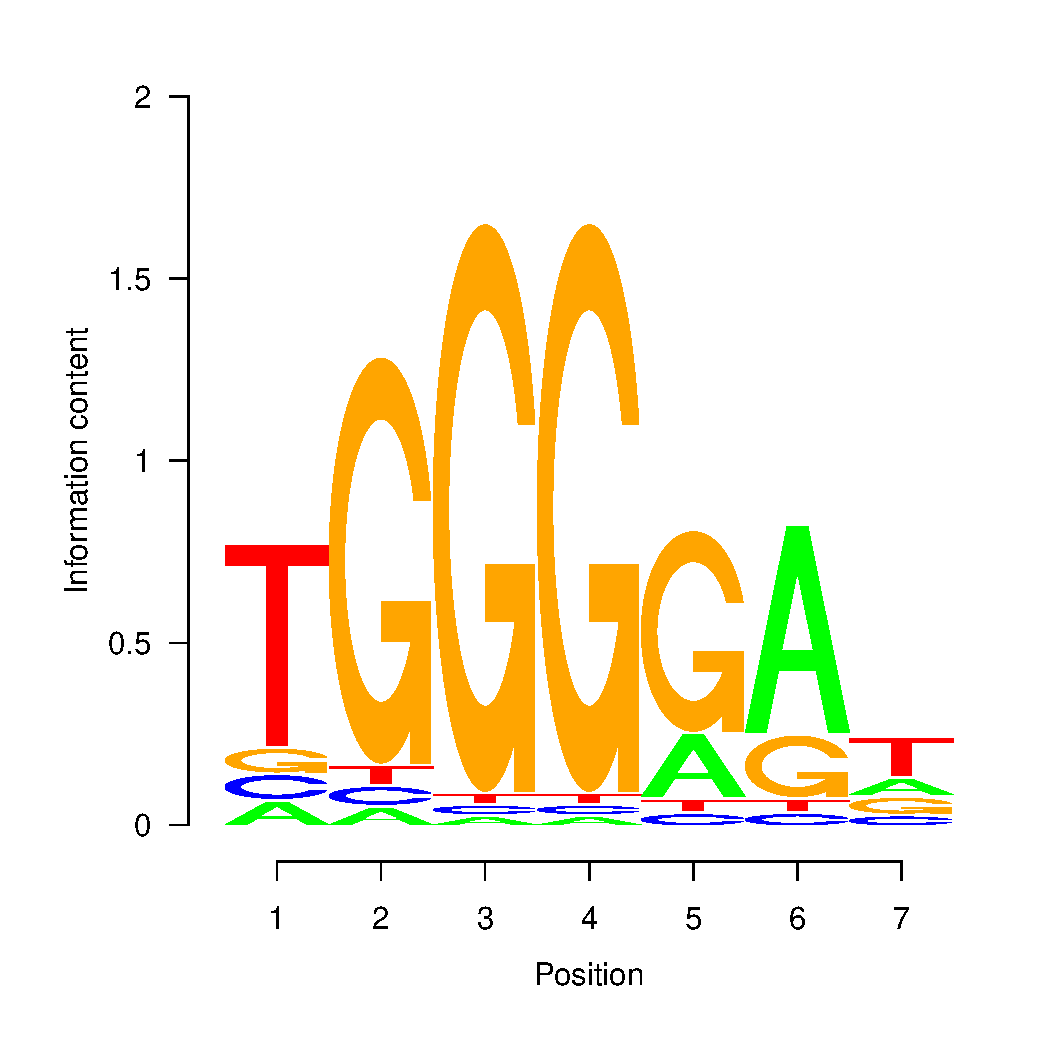
\includegraphics[height=0.8in]{./seqLogo/ESRP2_ugggrad.pdf} &ESPR2  is an epithelial cell-type-specific splicing regulator~\cite{Warzecha2009}.\\
 \hline
KHDRBS1 & AUAAAAV &  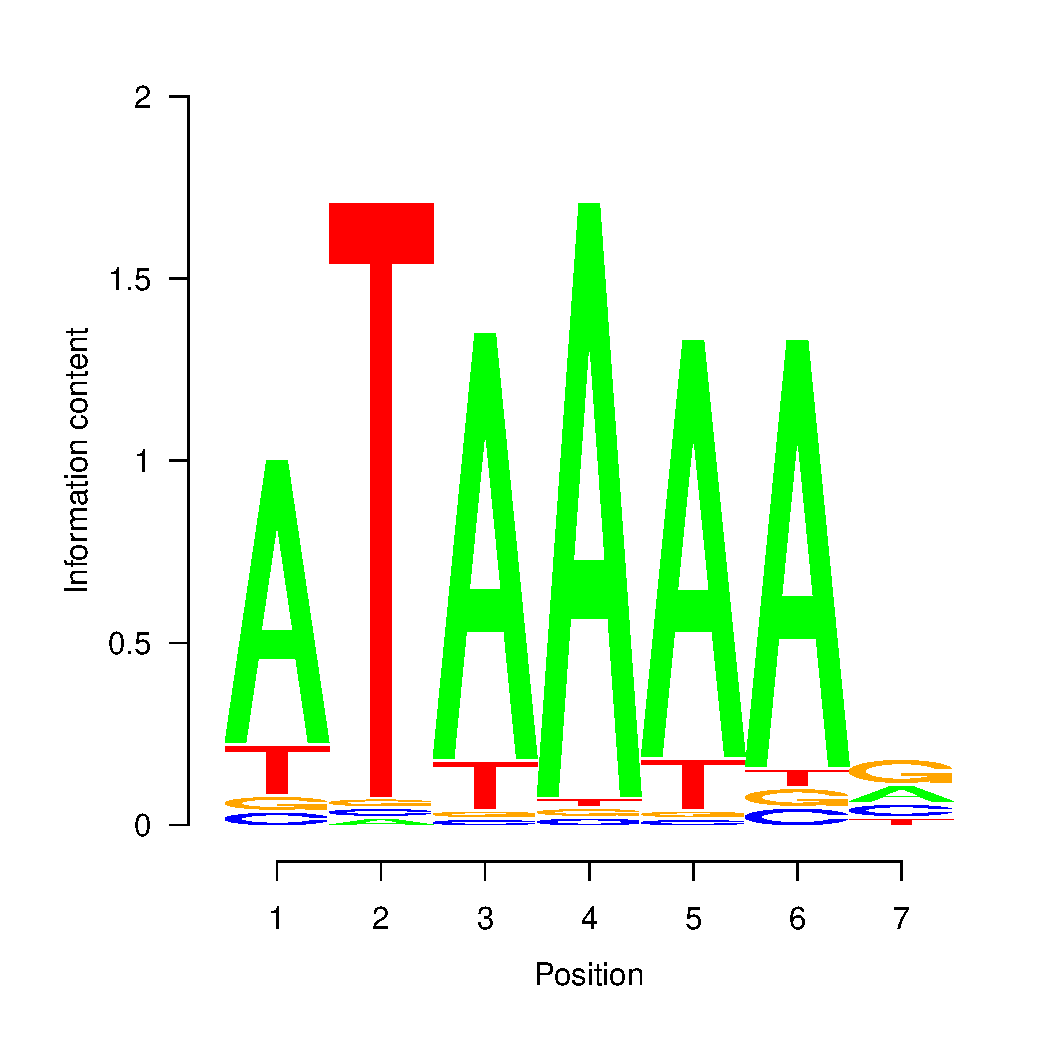
\includegraphics[height=0.8in]{./seqLogo/KHDRBS1_auaaaav.pdf} & \multirow{4}{6cm}{The KHDRBS proteins belong to the signal transduction activator of 
RNA (STAR) family of RNA-binding proteins that have several functions including a role in mediating alternative splicing~\cite{Matter2002}.  Quaking (QKI) is a conserved STAR (signal transduction and activation of RNA) family protein that plays an essential role during embryonic and postnatal development~\cite{Miguel2016}.} \\
KHDRBS2 & RAUAAAM & 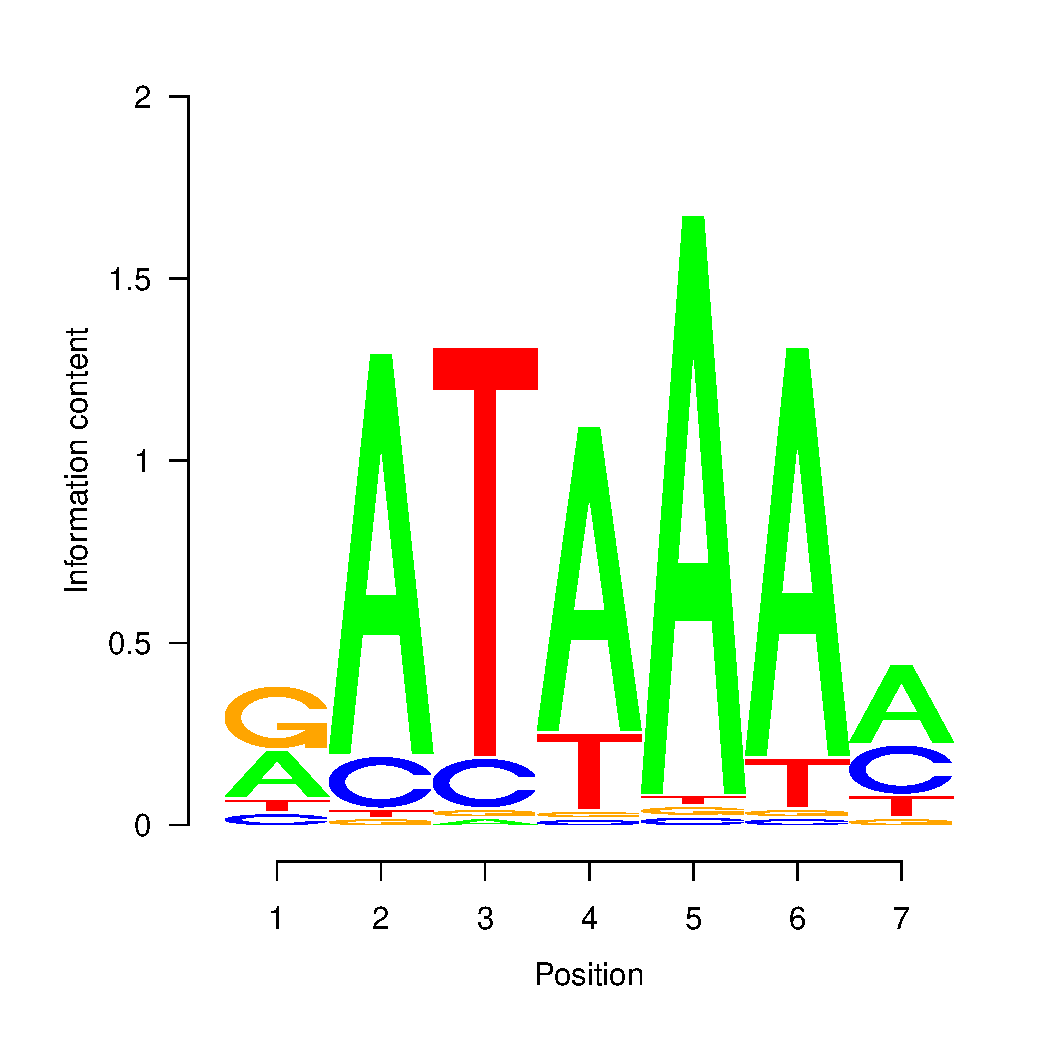
\includegraphics[height=0.8in]{./seqLogo/KHDRBS2_rauaaam.pdf}& \\
KHDRBS3 & AAAAV & 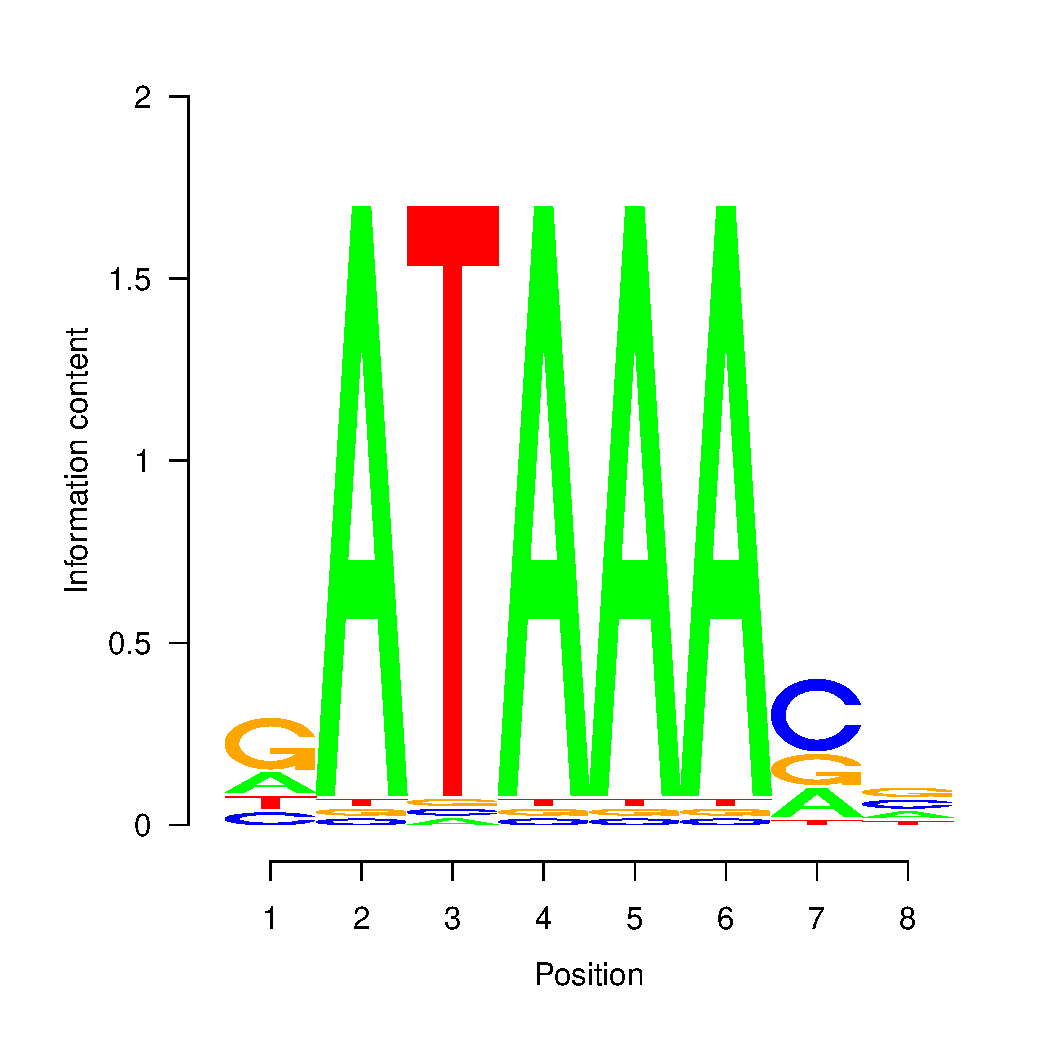
\includegraphics[height=0.8in]{./seqLogo/KHDRBS3_auaaav.pdf}& \\
QKI & ACUAAY & 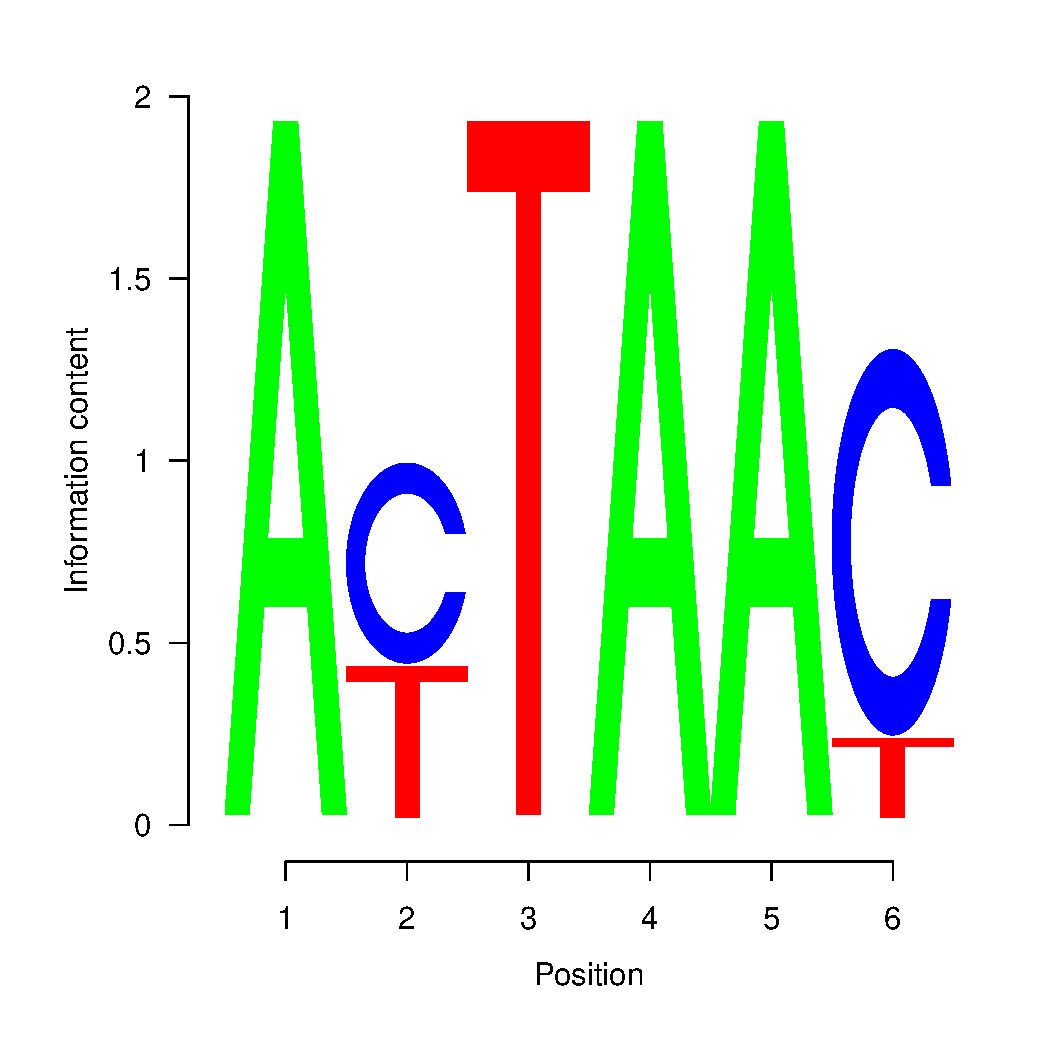
\includegraphics[height=0.8in]{./seqLogo/QKI_acuaay.pdf} & \\
\hline
MBNL1 & GCUUGC & 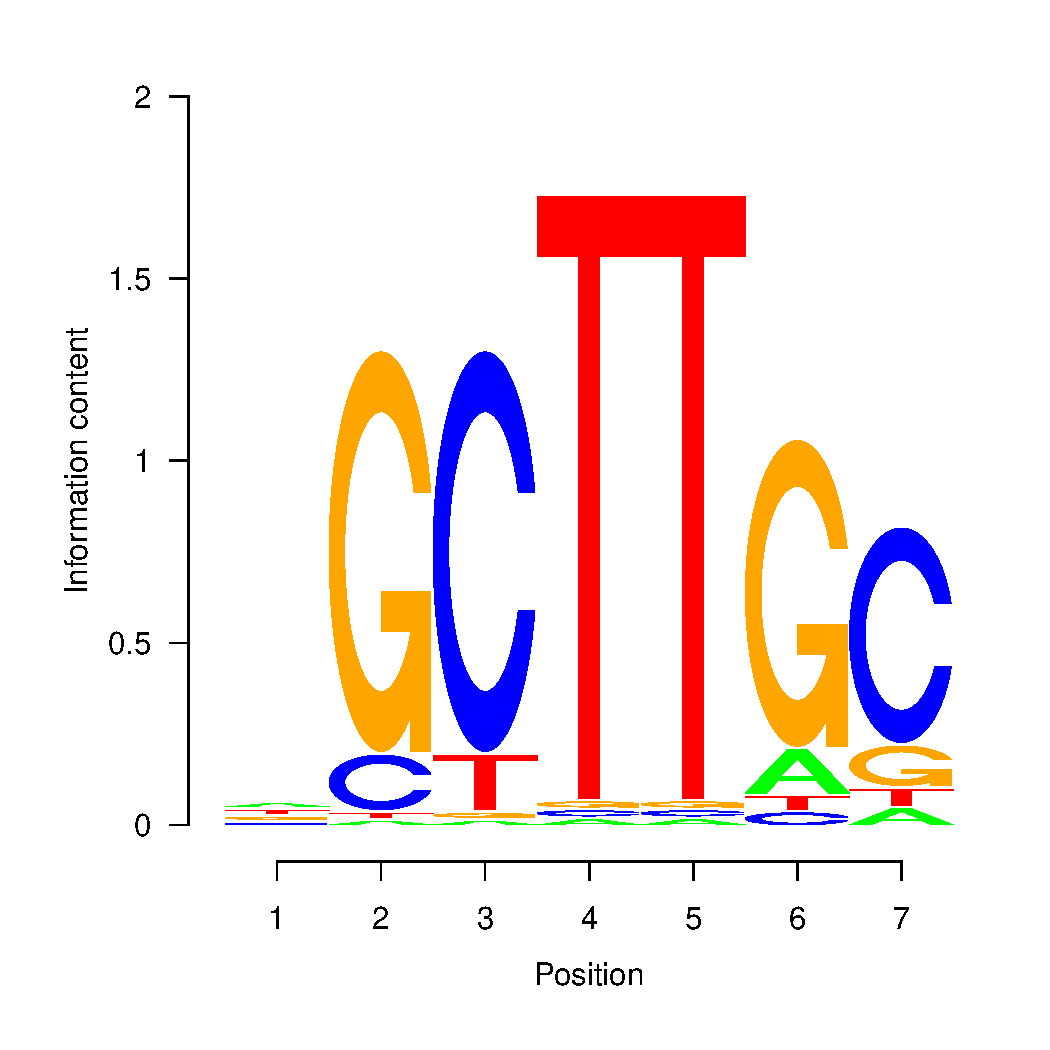
\includegraphics[height=0.8in]{./seqLogo/MBNL1_gcuugc.pdf} & The MBNL and CELF proteins act antagonistically to control the alternative splicing of specific exons during mammalian postnatal development~\cite{Yuan2007}. \\
\hline
PTBP1 & HYUUUYU  & 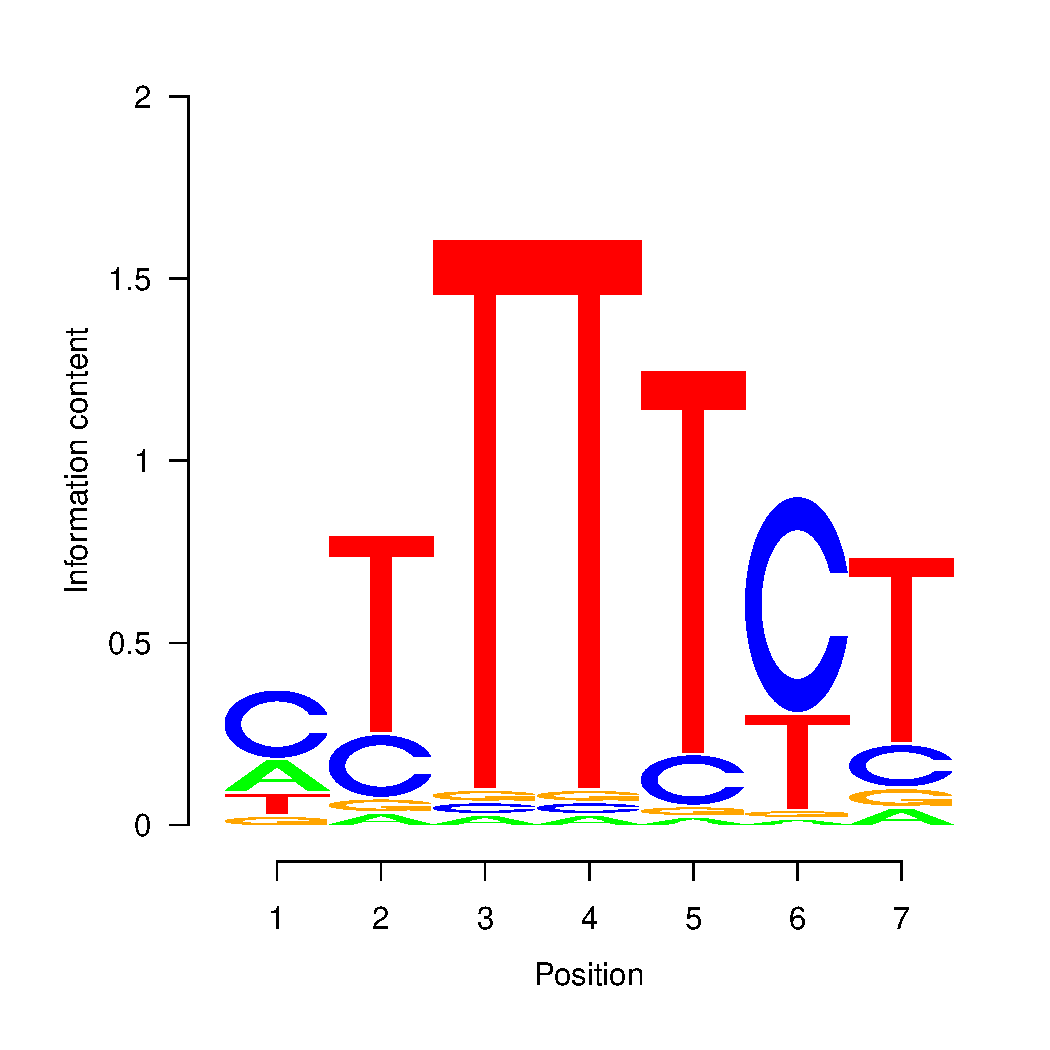
\includegraphics[height=0.8in]{./seqLogo/PTBP1_hyuuuyu.pdf} & PTPB1 is involved in fate conversion from fibroblast to cardiomyocyte and influences alternative splicing of numerous transcripts~\cite{Liu2017}.\\
\hline
RBM3 & RADACKA & 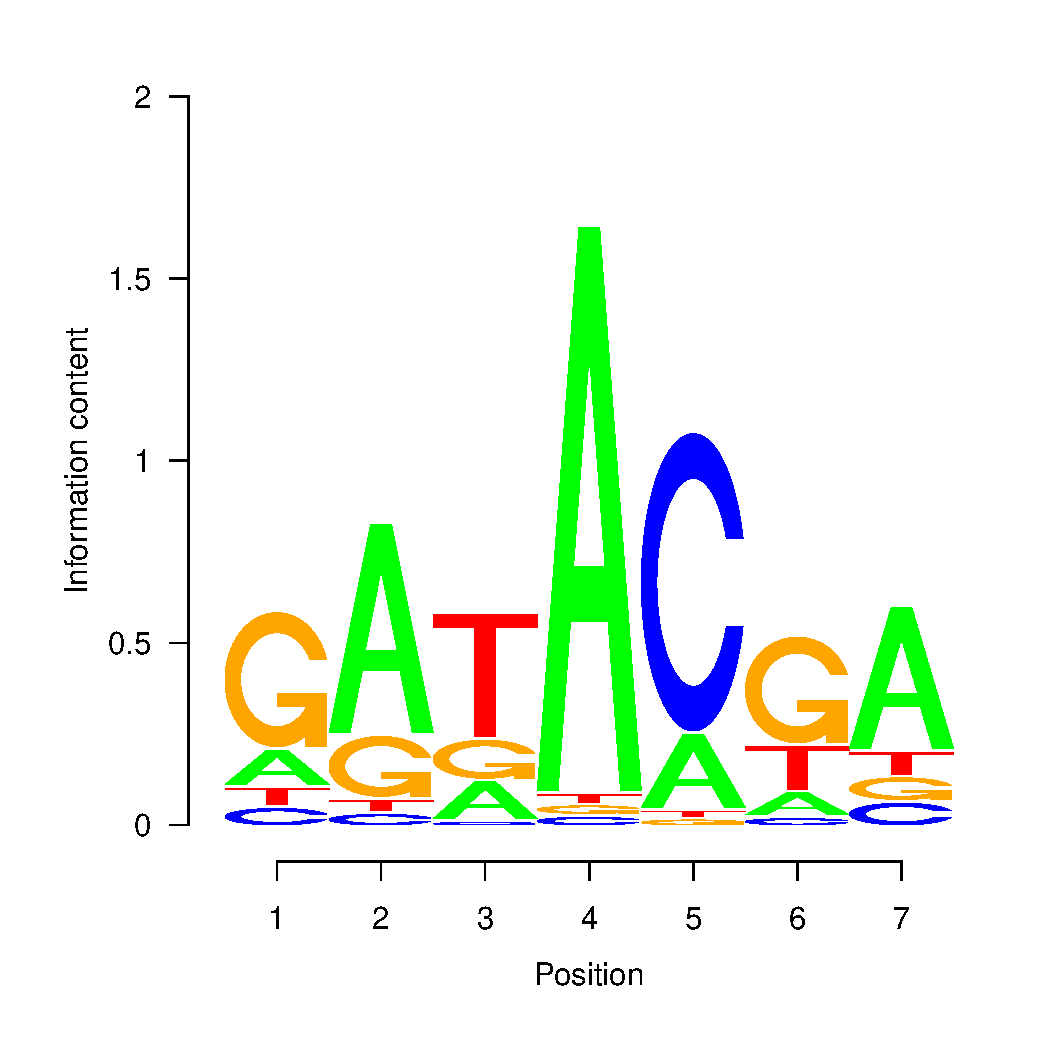
\includegraphics[height=0.8in]{./seqLogo/RBM3_radacka.pdf} &
 \multirow{12}{6cm}{
Genes of the RNA binding motif protein family, some of which are known to have a role in 
mediating alternative splicing: RBM10~\cite{Inoue2014} }\\
RBM4 & GCGCGSS & 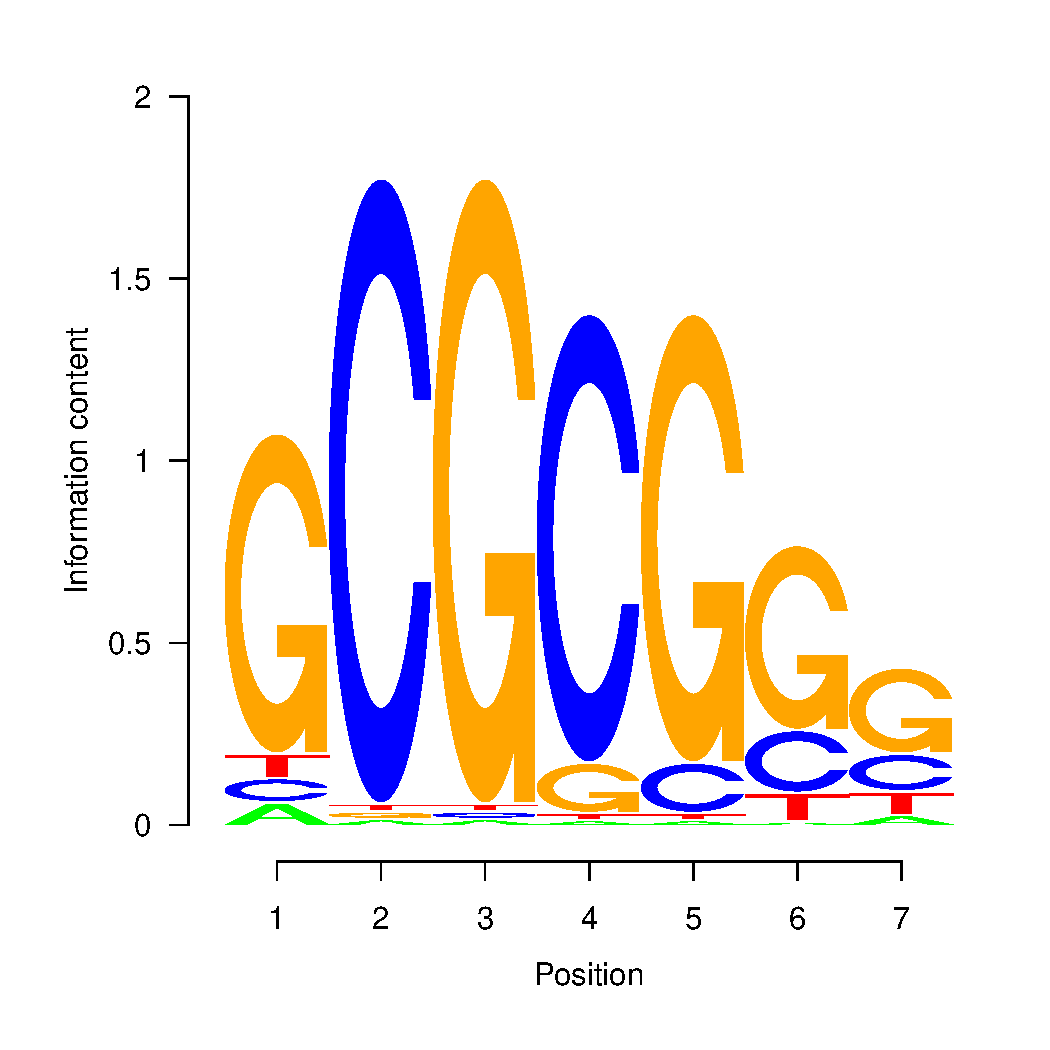
\includegraphics[height=0.8in]{./seqLogo/RBM4_gcgcgss.pdf} & \\
RBM5 & GARGGWR & 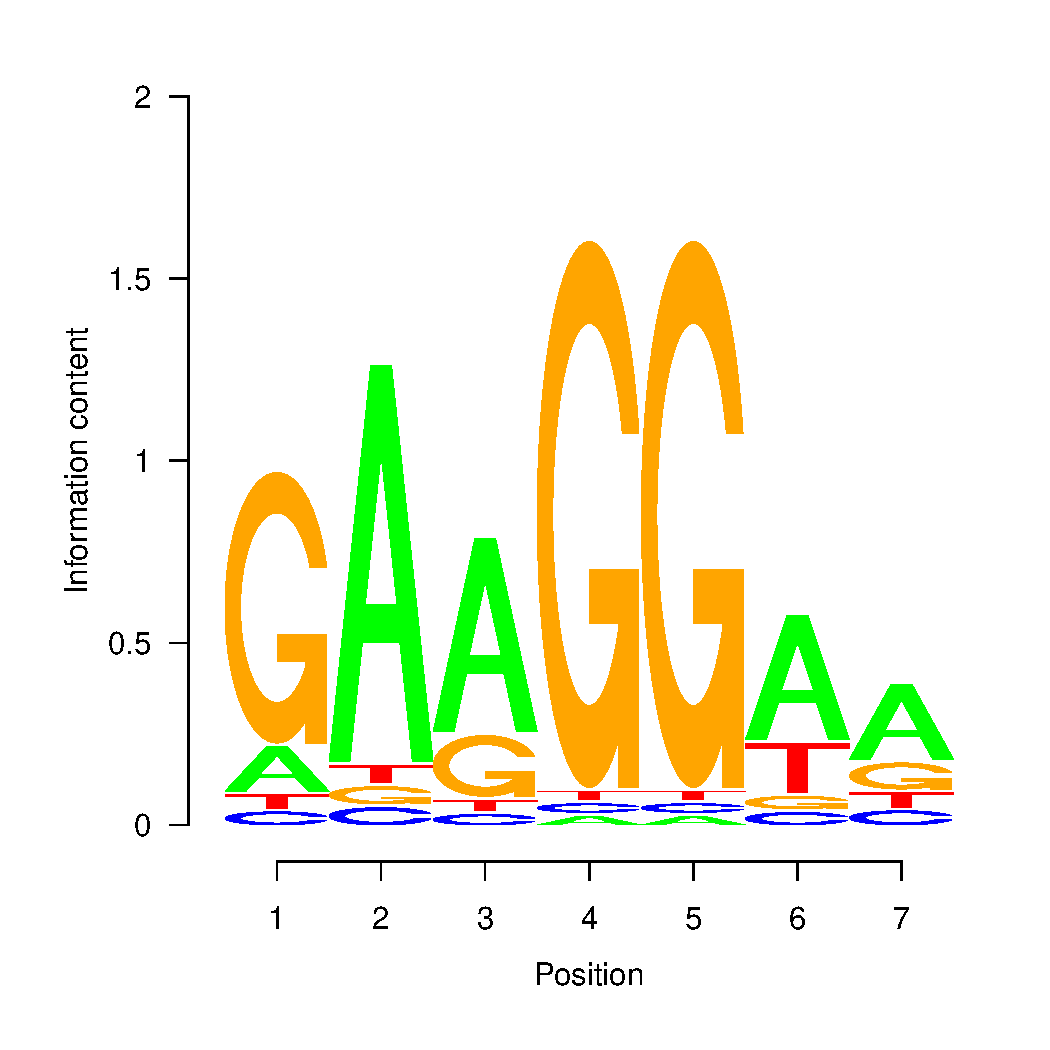
\includegraphics[height=0.8in]{./seqLogo/RBM5_garggwr.pdf} & \\
RBM6 & HAUCCAR & 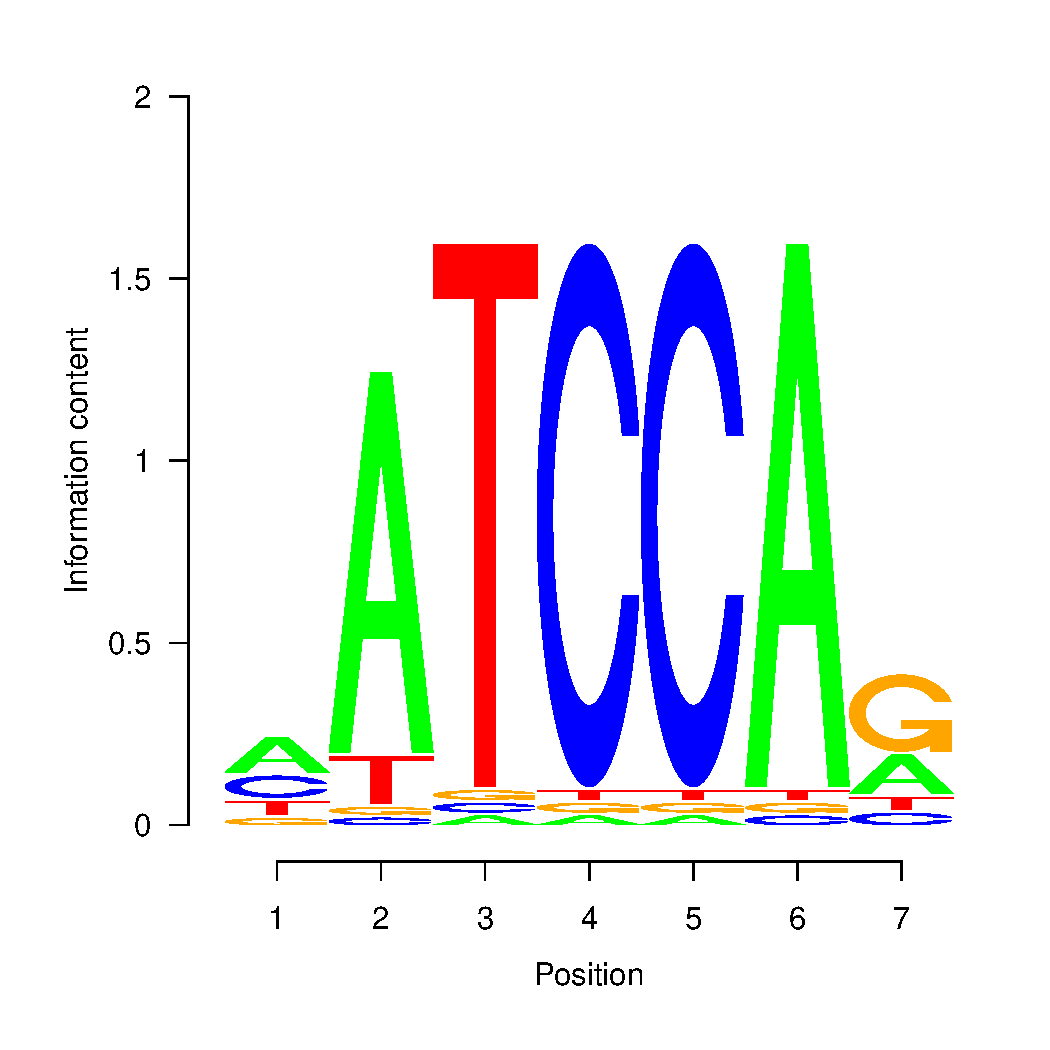
\includegraphics[height=0.8in]{./seqLogo/RBM6_hauccar.pdf} & \\
RBM8A  & RYGCGCB & 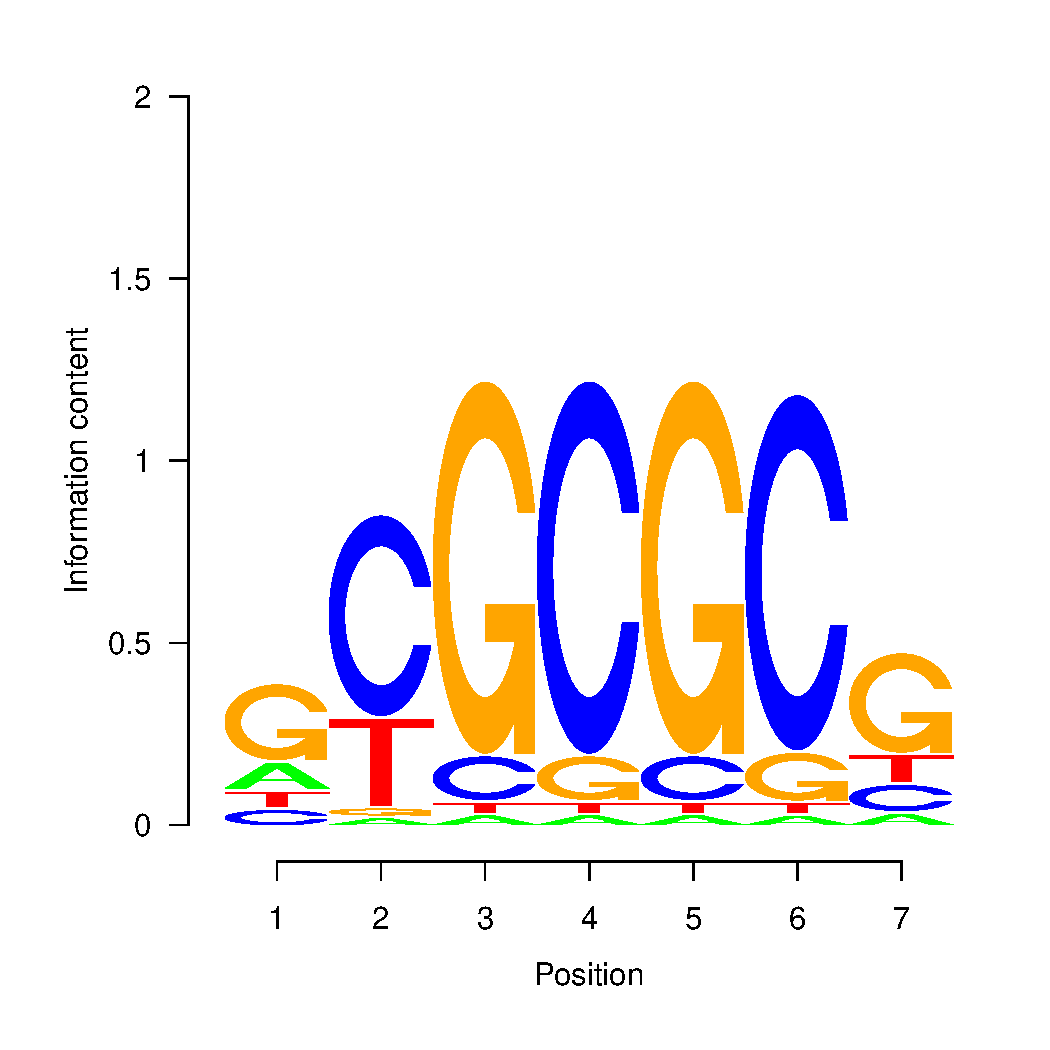
\includegraphics[height=0.8in]{./seqLogo/RBM8A_rygcgcb.pdf} & \\
RBM24 & WGWGUGD & 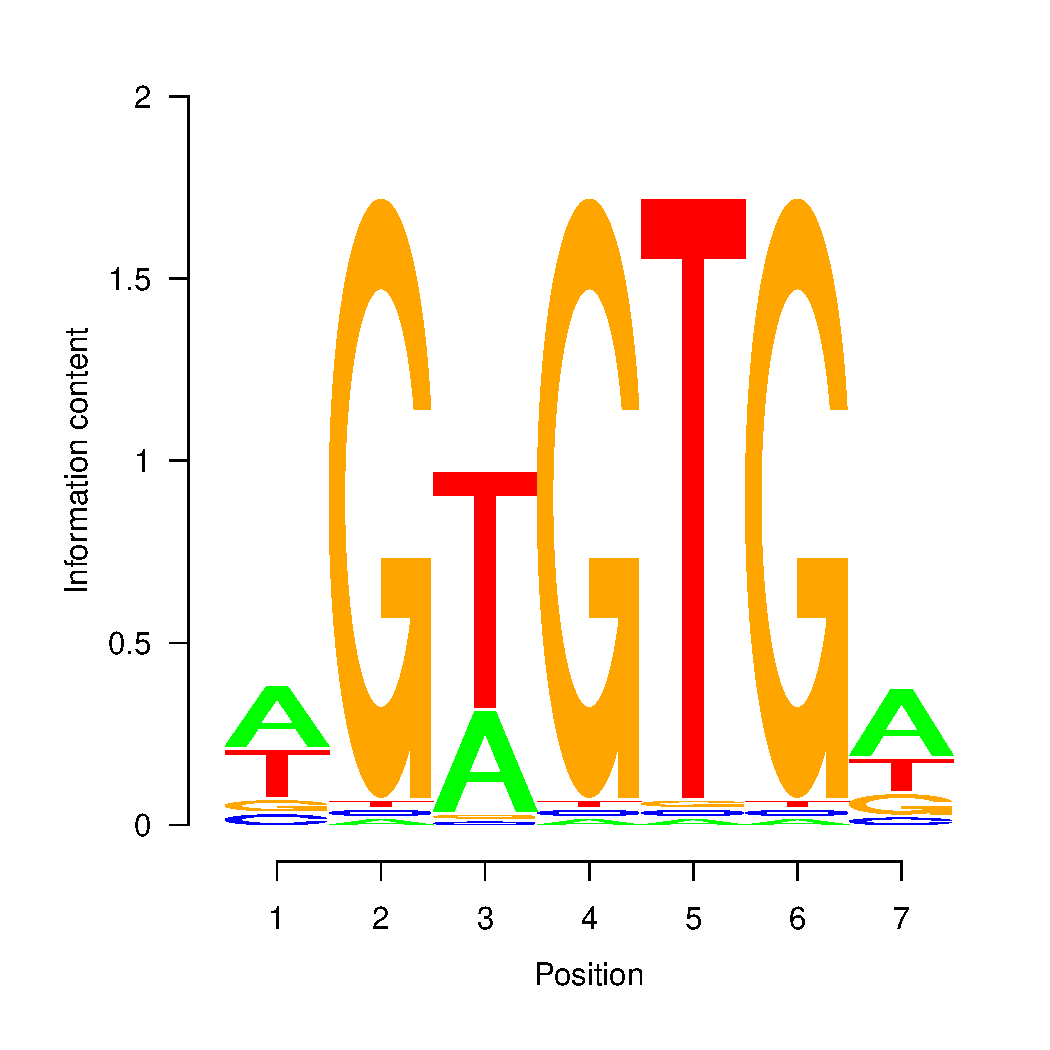
\includegraphics[height=0.8in]{./seqLogo/RBM24_wgwgugd.pdf}& \\
RBM41 & WUACWUK & 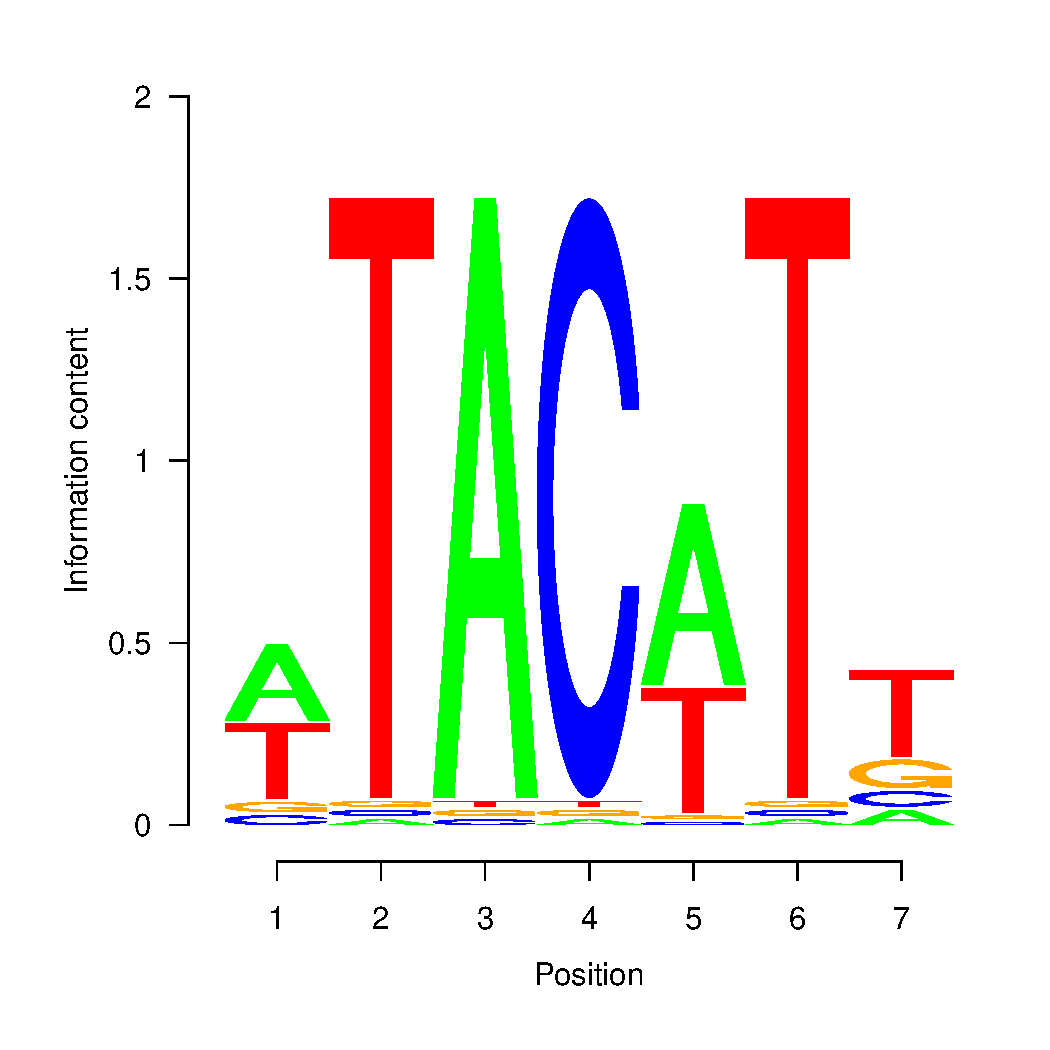
\includegraphics[height=0.8in]{./seqLogo/RBM41_wuacwuk.pdf}& \\   
RBM42 & AACUAMG & 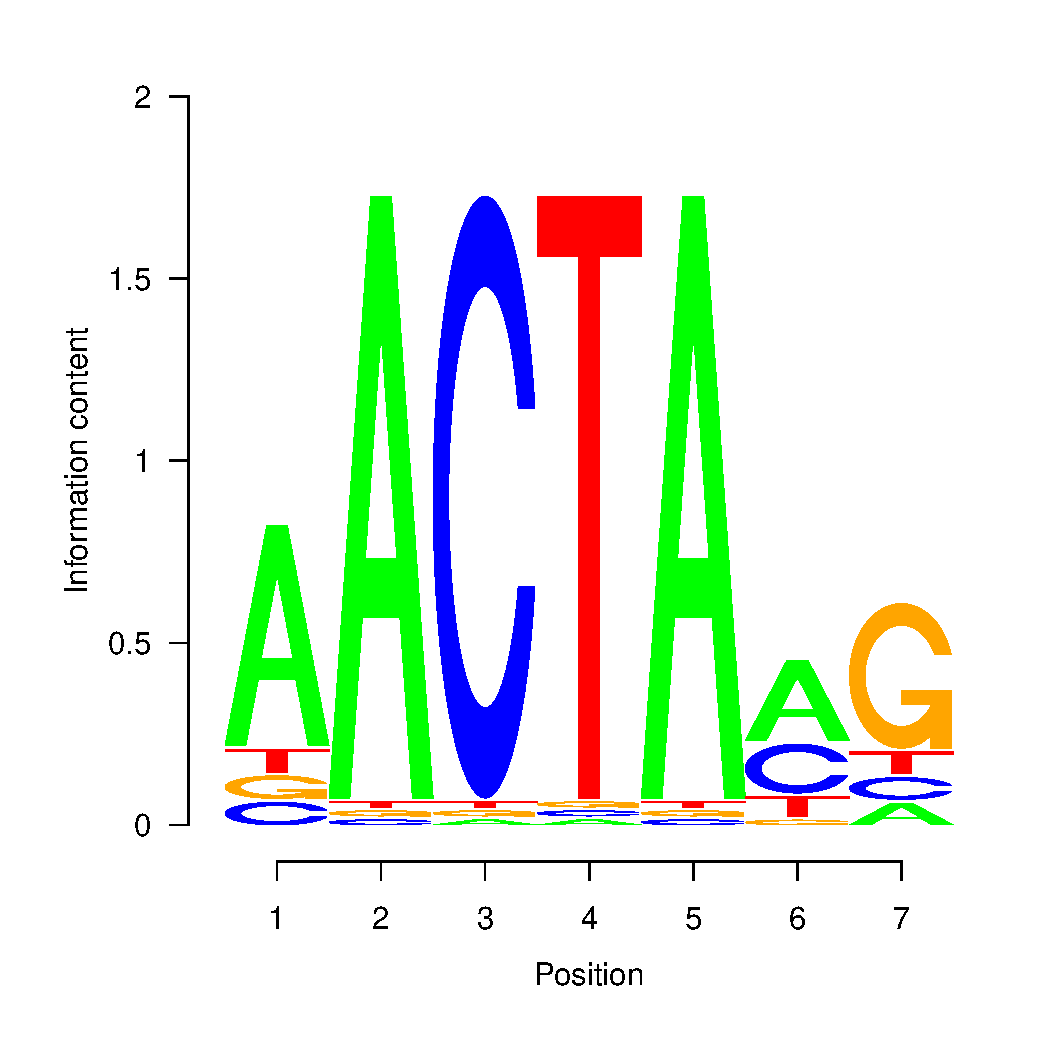
\includegraphics[height=0.8in]{./seqLogo/RBM42_aacuamg.pdf}& \\   
RBM45 & GACGAMV & 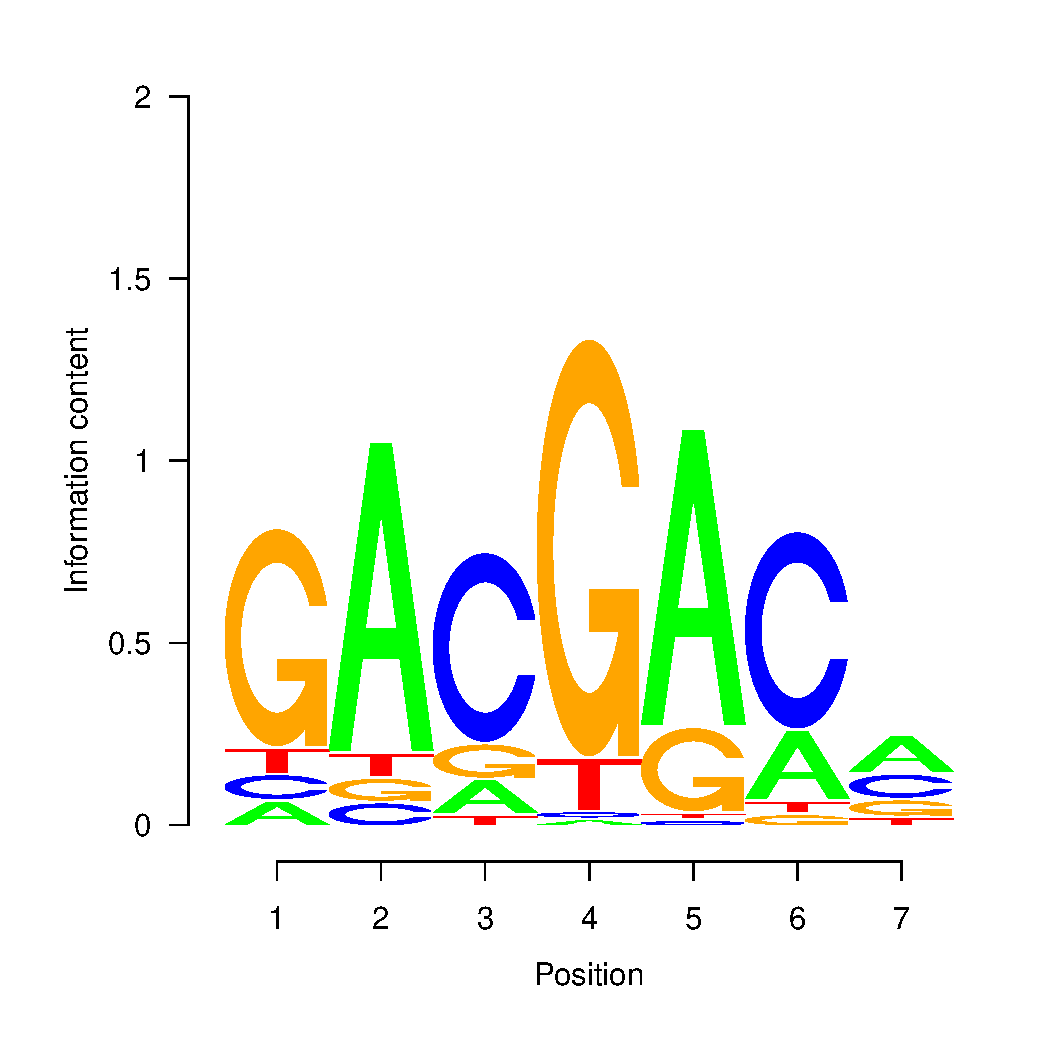
\includegraphics[height=0.8in]{./seqLogo/RBM45_gacgamv.pdf} & \\   
RBM46 & RAUSAWD & \includegraphics[height=0.8in]{./seqLogo/RBM46_rausawd.pdf} & \\   
RBMS1  & KAUAUAS & \includegraphics[height=0.8in]{./seqLogo/RBMS1_kauauas.pdf}& \\
RBMS3 &   &\includegraphics[height=0.8in]{./seqLogo/RBMS3_hauaua.pdf} & \\
\hline
SNRNP70 &RWUCAAG  & \includegraphics[height=0.8in]{./seqLogo/SNRNP70_rwucaag.pdf} &  snRNP70 is a key early regulator of 5' splice site selection~\cite{Carlson2015}\\
\hline
TIA1 & UUUUUBK & \includegraphics[height=0.8in]{./seqLogo/TIA1_uuuuubk.pdf} &  TIA-1 contains three RNA recognition motifs (RRM) and a carboxy-terminal glutamine-rich region and has diverse functions. TIA-1 and can  can act as a modulator of alternative splicing for human Fas receptor~\cite{Foerch2000}.











\end{longtable}
\end{center}

\bibliographystyle{unsrt}
\bibliography{/home/peter/GIT/Robinson-Lab/manuscripts/dimorph2AS/dimorph}

\end{document}
